\documentclass[10pt,oneside,a4paper]{article}

\usepackage{pdfpages}

\usepackage{algorithmic}
\usepackage{algorithm}
\usepackage{booktabs}
\usepackage{changepage}
\usepackage{enumitem}
\usepackage{geometry}
\usepackage{lscape}
\usepackage{hyperref}
\usepackage{siunitx}

\usepackage{caption}
\usepackage{subcaption}


%%%%%%%%%%%%%%%%%%%%%%%%%%%%%%%%%%%%%%%%%%%%%%%%%%%%%%%%%%%%%%%%%%%%%%%%%%%%%%%
% LaTeX preamble
%%%%%%%%%%%%%%%%%%%%%%%%%%%%%%%%%%%%%%%%%%%%%%%%%%%%%%%%%%%%%%%%%%%%%%%%%%%%%%%
% Encoding settings
\usepackage[utf8]{inputenc}
\usepackage[OT1]{fontenc}

% Paper size
\usepackage{a4}

% Headings
\usepackage{fancyhdr}

% More symbols
\usepackage{textcomp}\usepackage{gensymb}

% Math support for Times font
%\usepackage{txfonts}

% ISO date
\usepackage[english]{isodate}

% Multi column
\usepackage{multicol}

% Figures
\usepackage{graphicx}

% Subfigures (obsolete)
%\usepackage{subfigure}

% Bibliography
\usepackage[numbers]{natbib}

% Nicer tables
\usepackage{booktabs}
\usepackage{array}
\usepackage{multirow}

% Colors
\usepackage{color}
\usepackage{colortbl}
\definecolor{black}{rgb}{0,0,0}
\definecolor{white}{rgb}{1,1,1}
\definecolor{darkred}{rgb}{0.5,0,0}
\definecolor{darkgreen}{rgb}{0,0.5,0}
\definecolor{darkblue}{rgb}{0,0,0.5}

% Additional math functionality
\usepackage{amsmath}
\usepackage{amssymb}

% Nice fractions
\usepackage{nicefrac}

% Upper case greek letters
\usepackage{upgreek}

% ISO math notation
\usepackage{isomath}
\renewcommand{\vec}{\vectorsym}
\newcommand{\mat}{\matrixsym}

% Units
\usepackage{units}

% Rotated objects
\usepackage{rotating}

% Indent
\setlength{\parindent}{0em}

% Include PDF pages
\usepackage{pdfpages}
\includepdfset{pages={-}, frame=true, pagecommand={\thispagestyle{fancy}}}

% Headings
\rhead[\thepage]{\nouppercase{\rightmark}}
\lhead[\nouppercase{\leftmark}]{\thepage}
\cfoot{}

% Gantt chart
\usepackage{pgfgantt}

% Links (last package)
\PassOptionsToPackage{hyphens}{url}\usepackage{hyperref}

% Clever references (has to be loaded after hyperref)
\usepackage{cleveref}


%%%%%%%%%%%%%%%%%%%%%%%%%%%%%%%%%%%%%%%%%%%%%%%%%%%%%%%%%%%%%%%%%%%%%%%%%%%%%%%
% Title page
%%%%%%%%%%%%%%%%%%%%%%%%%%%%%%%%%%%%%%%%%%%%%%%%%%%%%%%%%%%%%%%%%%%%%%%%%%%%%%%
\begin{document}

\pagestyle{empty}
 
\begin{center}
\hspace{0.02\textwidth}
\parbox[c][\textheight][t]{0.97\textwidth}{
\begin{center}

% logos
\vspace*{-3.2cm}

\hspace*{-3.5cm}
\begin{tabular}{lp{4cm}r}
\multirow{3}{8cm}{\includegraphics[height=1.5cm]{images/eth_logo.pdf}} & & \multirow{3}{6cm}{\vspace{-0.6cm}\begin{flushright}
\includegraphics[height=0.8cm]{images/relab_logo.pdf}\\Rehabilitation Engineering Laboratory\\
\end{flushright}}\\
 & & \\
 & & \\
 & & \\
\end{tabular}

% line
\hspace*{-124pt}
\textcolor{gray}{\rule{595pt}{0.1pt}}

\vspace{22cm}

% line
\hspace*{-124pt}
\textcolor{gray}{\rule{595pt}{0.1pt}}

\vspace*{0.7cm}
\hspace*{-3.3cm}
\begin{tabular}{p{8cm}p{6cm}r}
Monika Zbytniewska & &\\
Rehabilitation Engineering Laboratory & &\\
ETH Zurich  & &\\
BAA, Lengghalde 5 & &\\
8008 Zurich & &\\
Switzerland & & \today
\end{tabular}

% title	
\vspace{-21cm}	
{\Huge \bf ETH MIKE - Manual \par}


\vspace{3cm}
{\hspace*{-1.2cm}	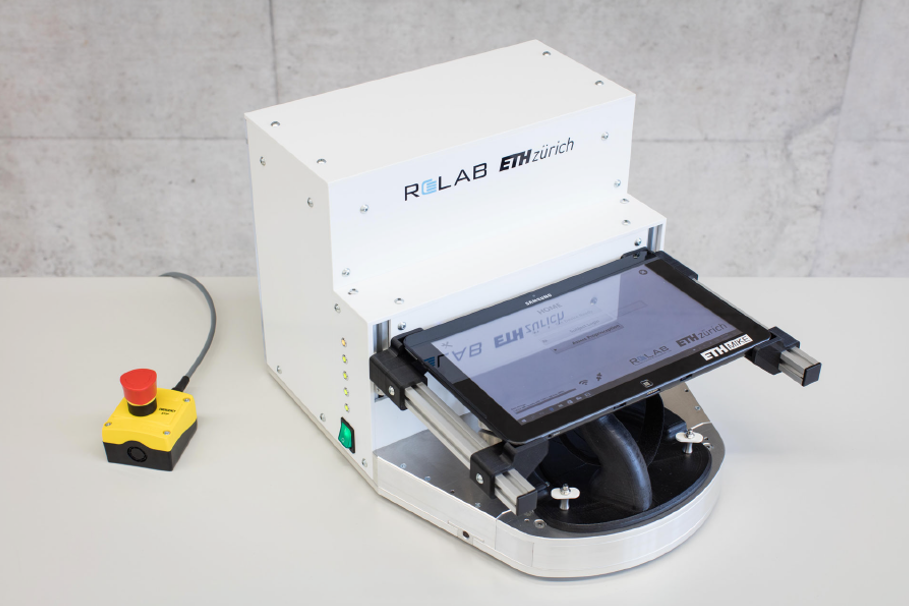
\includegraphics[height=10cm]{images/Hardware/ETHMIKE2.png}}

\end{center}
}
\end{center}

\clearpage

\pagestyle{plain}
\pagenumbering{arabic}

%%%%%%%%%%%%%%%%%%%%%%%%%%%%%%%%%%%%%%%%%%%%%%%%%%%%%%%%%%%%%%%%%%%%%%%%%%%%%%%
% Table on contents
%%%%%%%%%%%%%%%%%%%%%%%%%%%%%%%%%%%%%%%%%%%%%%%%%%%%%%%%%%%%%%%%%%%%%%%%%%%%%%%

% Table of Contents depth (TODO change if necessary)
\setcounter{tocdepth}{2}

\tableofcontents
\cleardoublepage


%%%%%%%%%%%%%%%%%%%%%%%%%%%%%%%%%%%%%%%%%%%%%%%%%%%%%%%%%%%%%%%%%%%%%%%%%%%%%%%
% Content
%%%%%%%%%%%%%%%%%%%%%%%%%%%%%%%%%%%%%%%%%%%%%%%%%%%%%%%%%%%%%%%%%%%%%%%%%%%%%%%


\section{List of all Parts}
The robot ETH MIKE comes with the parts shown in Figure \ref{fig:parts} and Table \ref{tab:parts} below.

\begin{figure}[h!]
\begin{center}
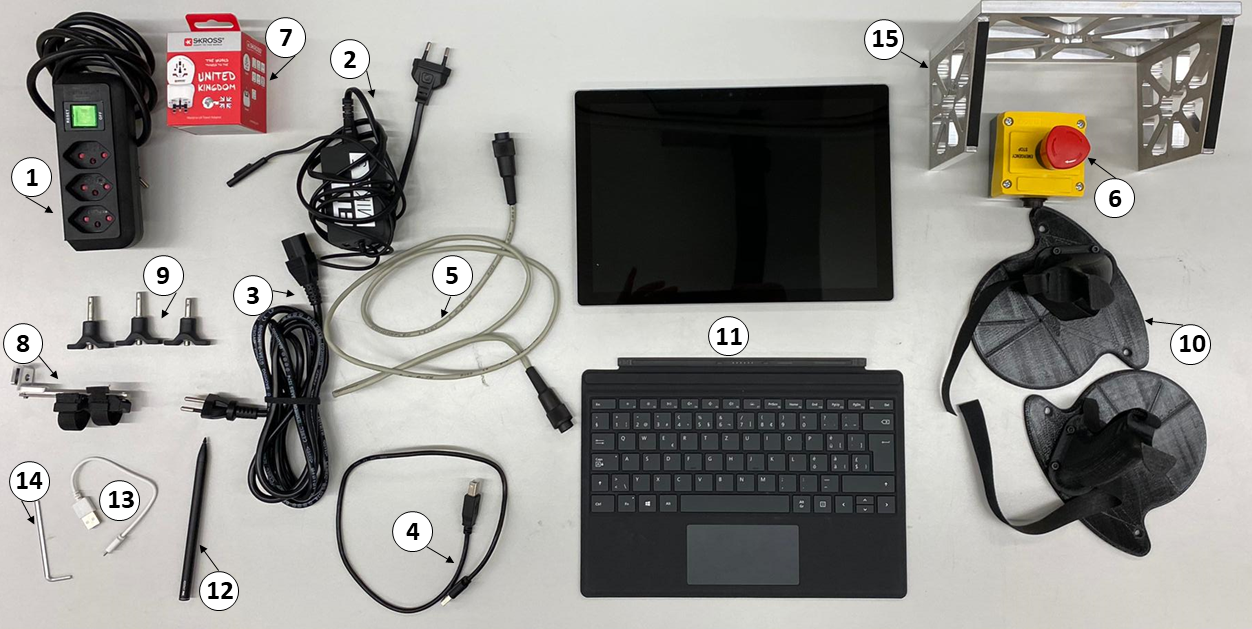
\includegraphics[width=\columnwidth]{images/Hardware/parts_annotated.png}
\caption{Overview of all components of the ETH MIKE robot.}
\label{fig:parts}
\end{center}
\end{figure}

\begin{table}[h!]
\centering
\begin{tabular}{lll}
Number & Item & Quantity\\
\hline
1 & Extension cable (power strip) & 1 \\
2 & Tablet power supply & 1 \\
3 & Robot main power cable & 1 \\
4 & USB connection cable between tablet and robot & 1 \\
5 & Emergency stop button cable & 1 \\
6 & Emergency stop button & 1 \\
7 & Adapter (UK/EU depending on delivery destination) & 1 \\
8 & Finger module & 1 \\
9 & Pins for the finger module (short) and handles (long) & 1 short 2 long \\
10 & Handles (left- and right-hand version) & 2 \\
11 & Tablet computer and keyboard & 1 \\
12 & Tablet pen & 1 \\
13 & Cable to charge the tablet pen & 1 \\
14 & Allen key & 1 \\
15 & Incline plane & 1 \\
16 & End-effector lock (not on picture) & 1 \\
17 & Protection pin (not on picture) & 1 \\
19 & Leukotape classic (not on picture) & 1 \\
20 & Tricofix (not on picture) & 1 \\
21 & Wrist splint (not on picture) & 1 \\
\end{tabular}
\caption{List of all components of the ETH MIKE robot.}
\label{tab:parts}
\end{table}

\newpage
\section{Setup}

\subsection{ETH MIKE Full Setup}
Below you can see how the ETH MIKE looks like when it’s fully set-up. In the following steps, you will be guided through the process how to get to this stage.

\begin{figure}[h!]
\centering
\begin{subfigure}[b]{0.48\textwidth}
	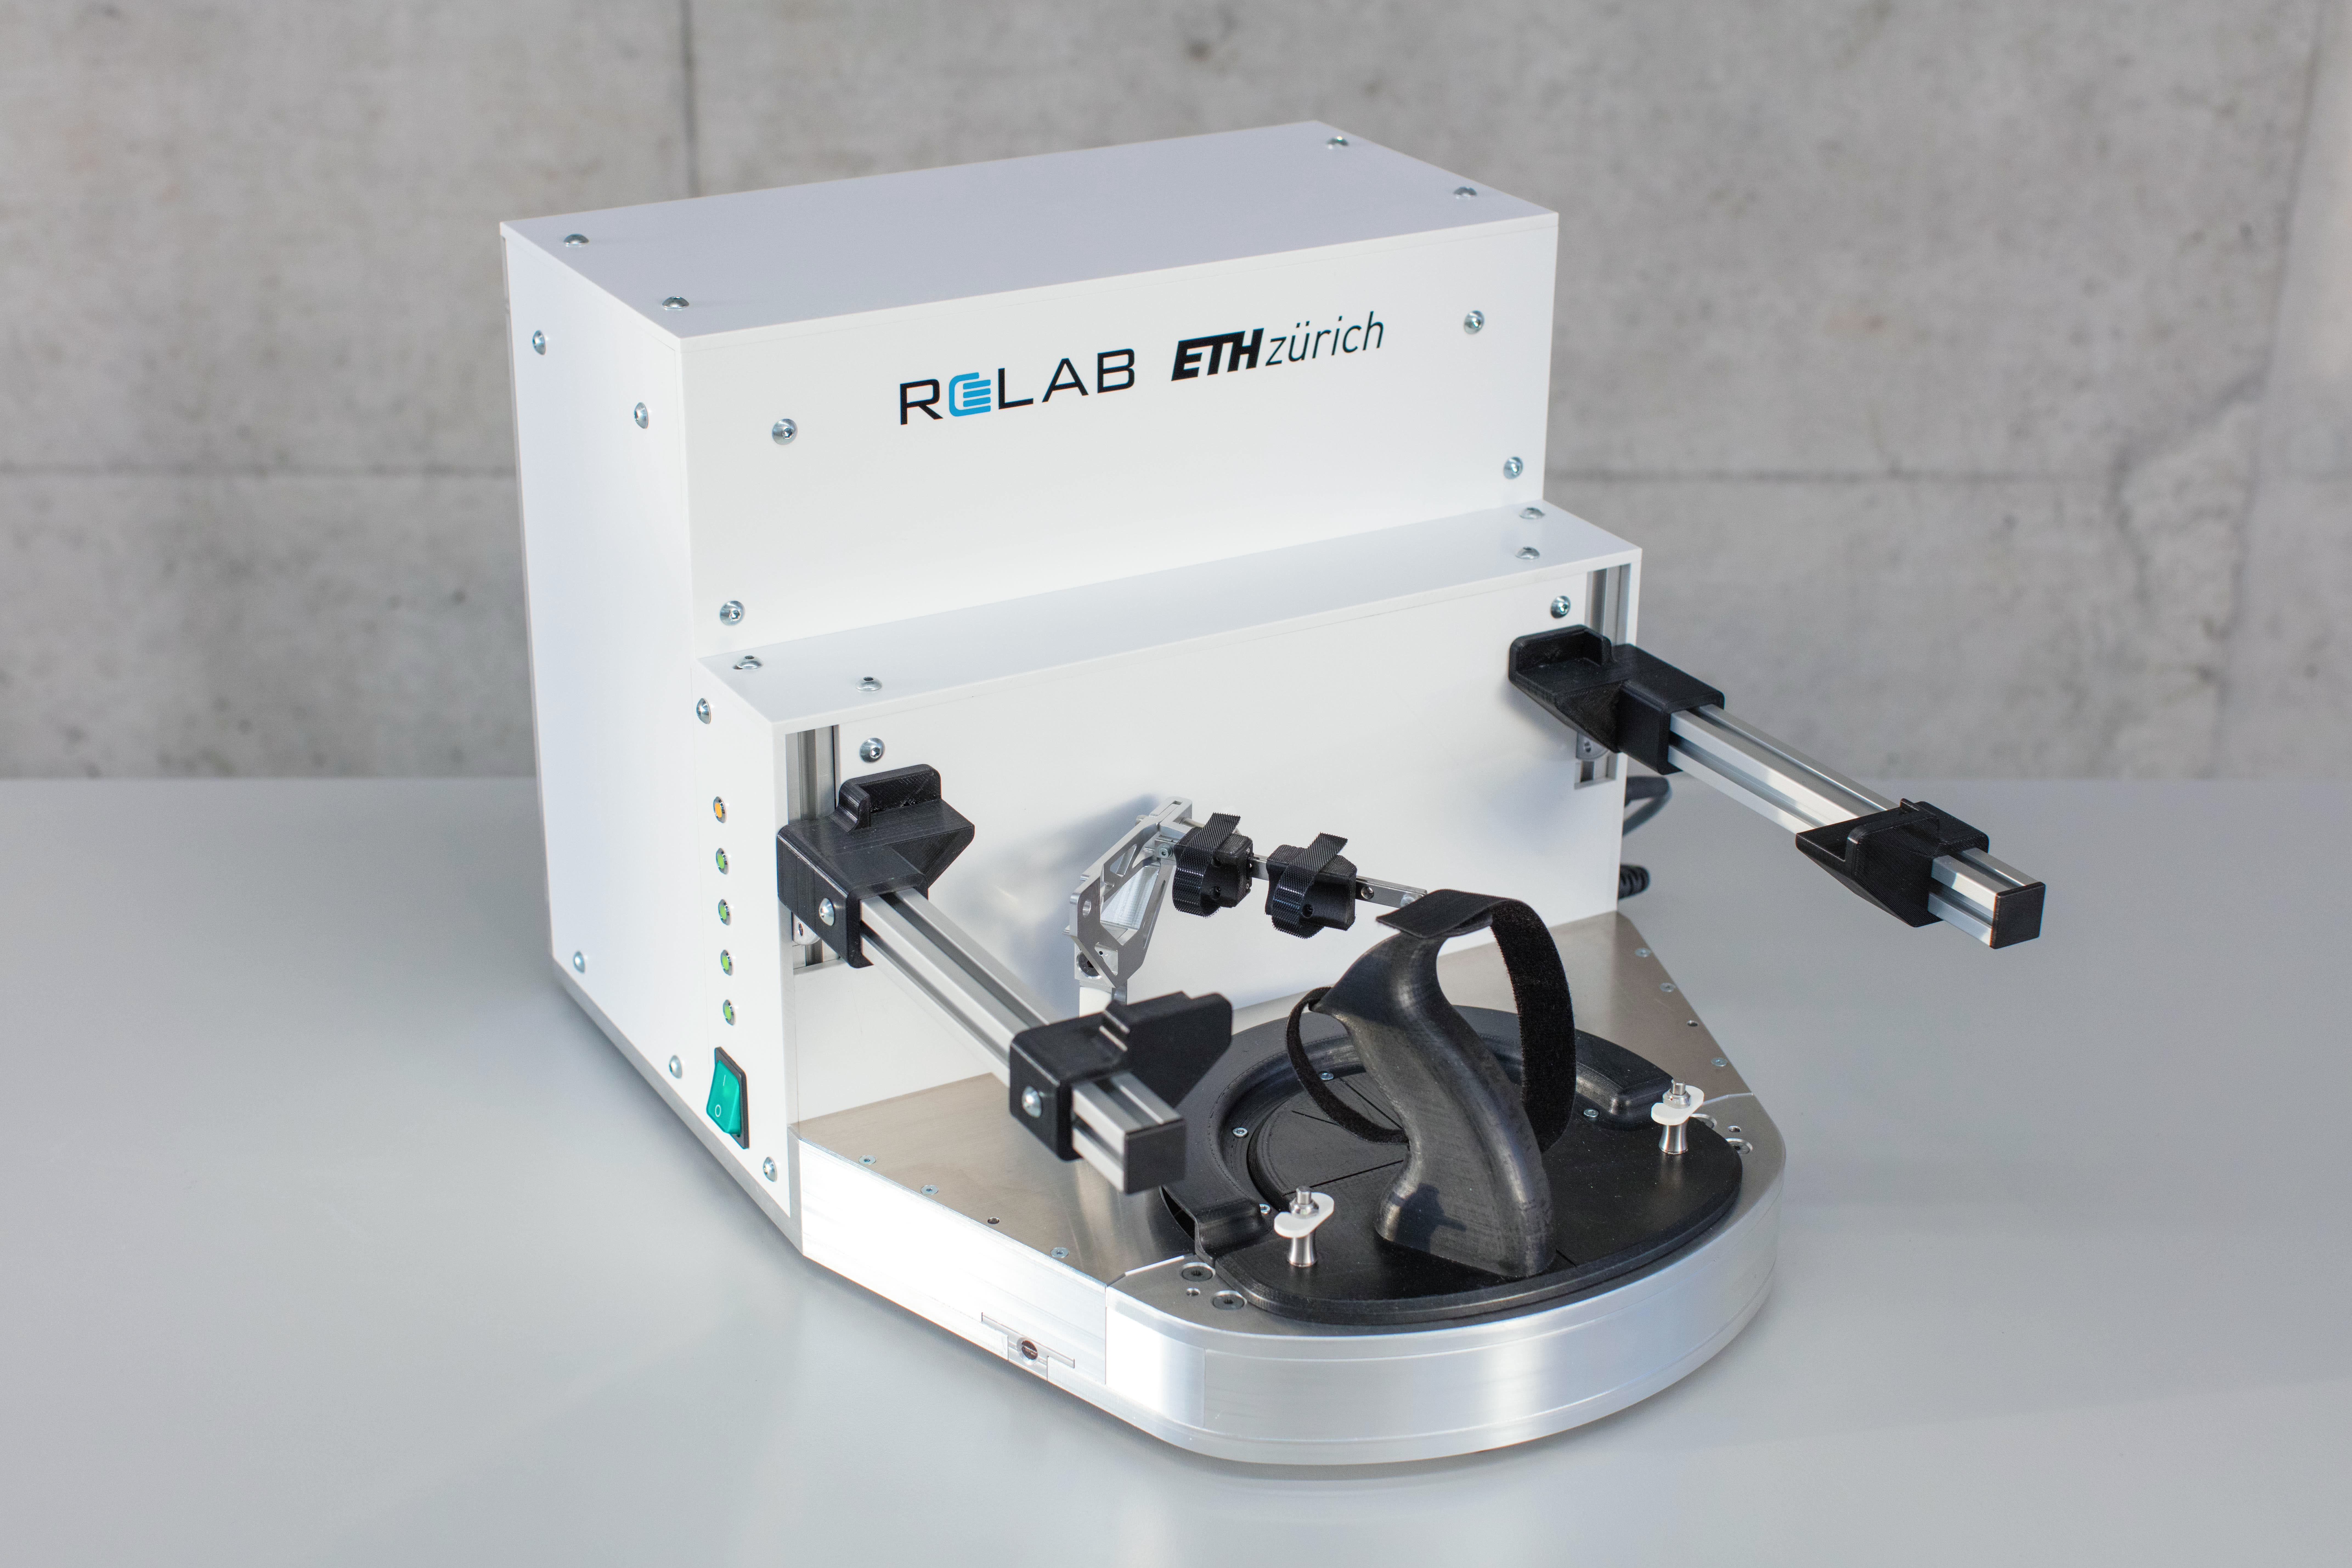
\includegraphics[height=4cm]{images/Hardware/ETHMIKE.jpg}
\end{subfigure}
\hfill
\begin{subfigure}[b]{0.48\textwidth}
	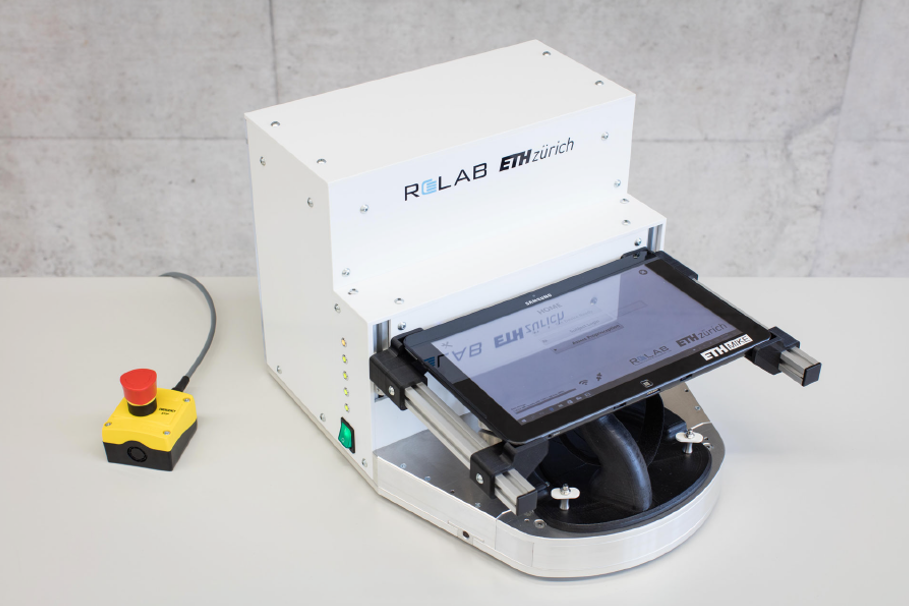
\includegraphics[height=4cm]{images/Hardware/ETHMIKE2.png}
\end{subfigure}
\caption{ETH MIKE full setup – with and without the tablet computer placed on the dedicated rails.}
\label{fig:mike}
\end{figure}

\subsection{Cables}
Firstly, place the extension cable (\#1 Table \ref{tab:parts}) within reach. Then, insert the robot main power cable (\#3 Table \ref{tab:parts}) to the input on the robot (\#1 Figure \ref{fig:cables}) and its other side to the extension cable. As the next step, connect the emergency stop button with its cable (\#5 and \#6 Table \ref{tab:parts}) and insert the other side of that cable to the robot (\#2 Figure \ref{fig:cables}). Next, connect the USB cable to the robot (\#3 Figure \ref{fig:cables}) and to the USB input port of the tablet. Finally, connect the power supply of the tablet to the tablet and to the extension cable. Power the extension cable using the adapter (\#7 Table \ref{tab:parts}). 

\begin{figure}[h!]
\begin{center}
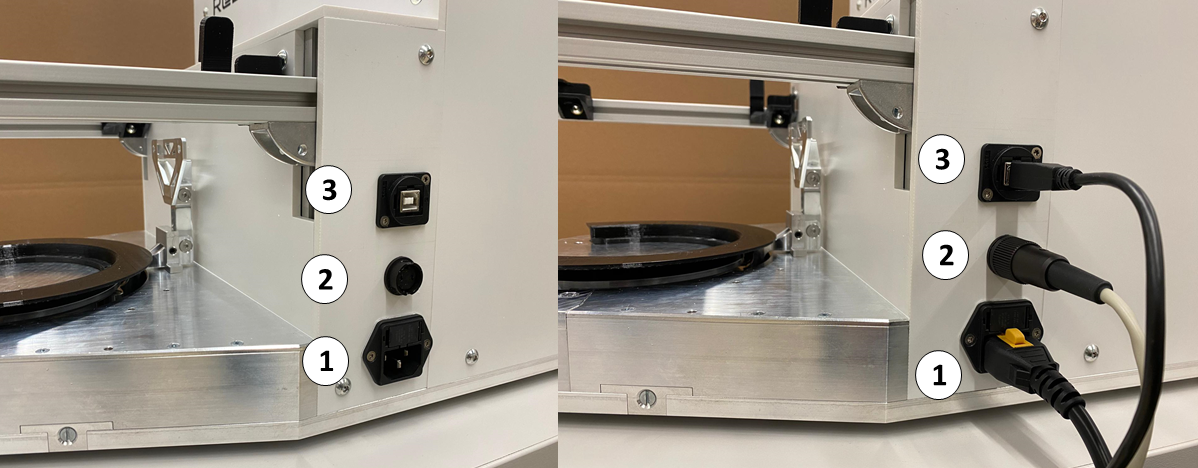
\includegraphics[width=\columnwidth]{images/Hardware/CablesBoth.png}
\caption{How to connect power cable and emergency button to the robot.}
\label{fig:cables}
\end{center}
\end{figure}

\subsection{Emergency Button}
The emergency stop button (\#6 Table \ref{tab:parts}) has two states: released and pressed (Figure \ref{fig:EmergencyButton}). Pressing the emergency button cuts the current to the actuation of the robot and should only be used in emergencies. To re-enable the actuation, the emergency button needs to be released by turning the red knob, and the robot needs to be restarted. 

\begin{figure}[h!]
\begin{center}
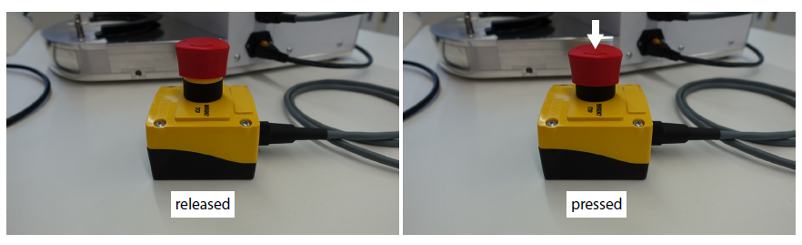
\includegraphics[width=\columnwidth]{images/Hardware/EmergencyButton.png}
\caption{Emergency button – released and pressed.}
\label{fig:EmergencyButton}
\end{center}
\end{figure}

\subsection{Hand and Finger Interface}
In order to prepare the hand and finger interface, first place the finger module (\#8 Table \ref{tab:parts}) as in shown in Figure \ref{fig:HandPlacement} and secure it with the shorter pin. Then, place one of the handles and secure it with two longer pins. Check Figure \ref{fig:HandPlacement} for demonstration of hand placement. The placement of the hand into the system is demonstrated in detail in \href{https://www.youtube.com/watch?v=jmWdwJ00onU&t=1s&ab_channel=RELABETHZ}{this video}. 

\begin{figure}[h!]
\centering
\begin{subfigure}[b]{0.48\textwidth}
	\centering
	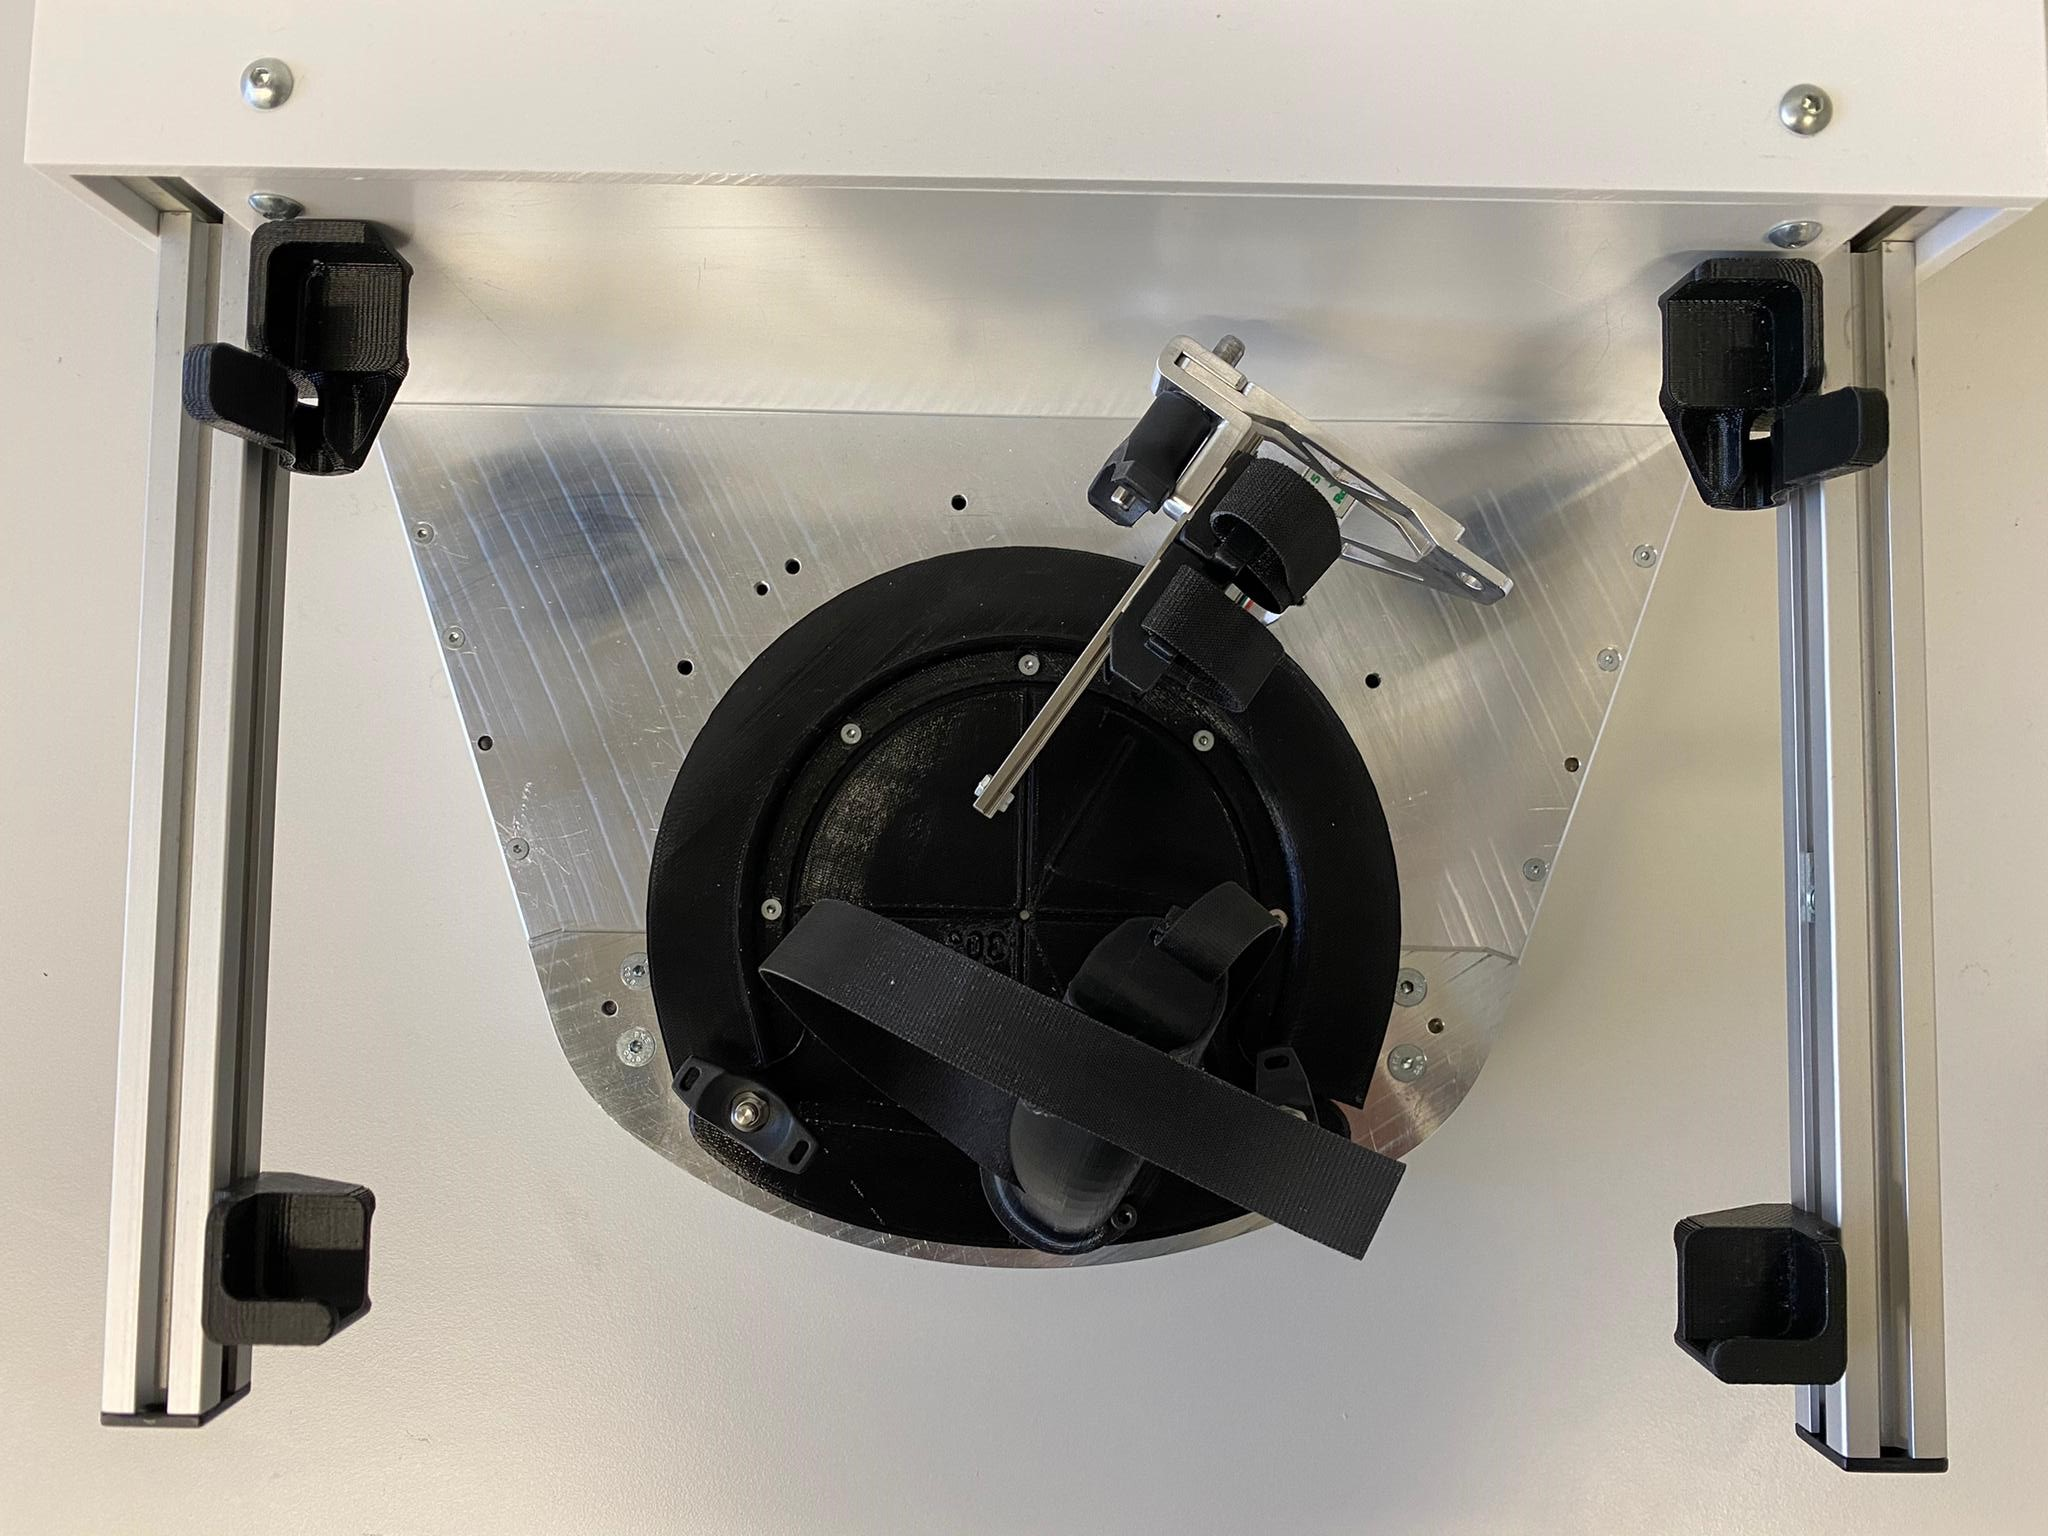
\includegraphics[width=\textwidth]{images/Hardware/leftside.jpeg}
\end{subfigure}
\hfill
\begin{subfigure}[b]{0.48\textwidth}
	\centering
	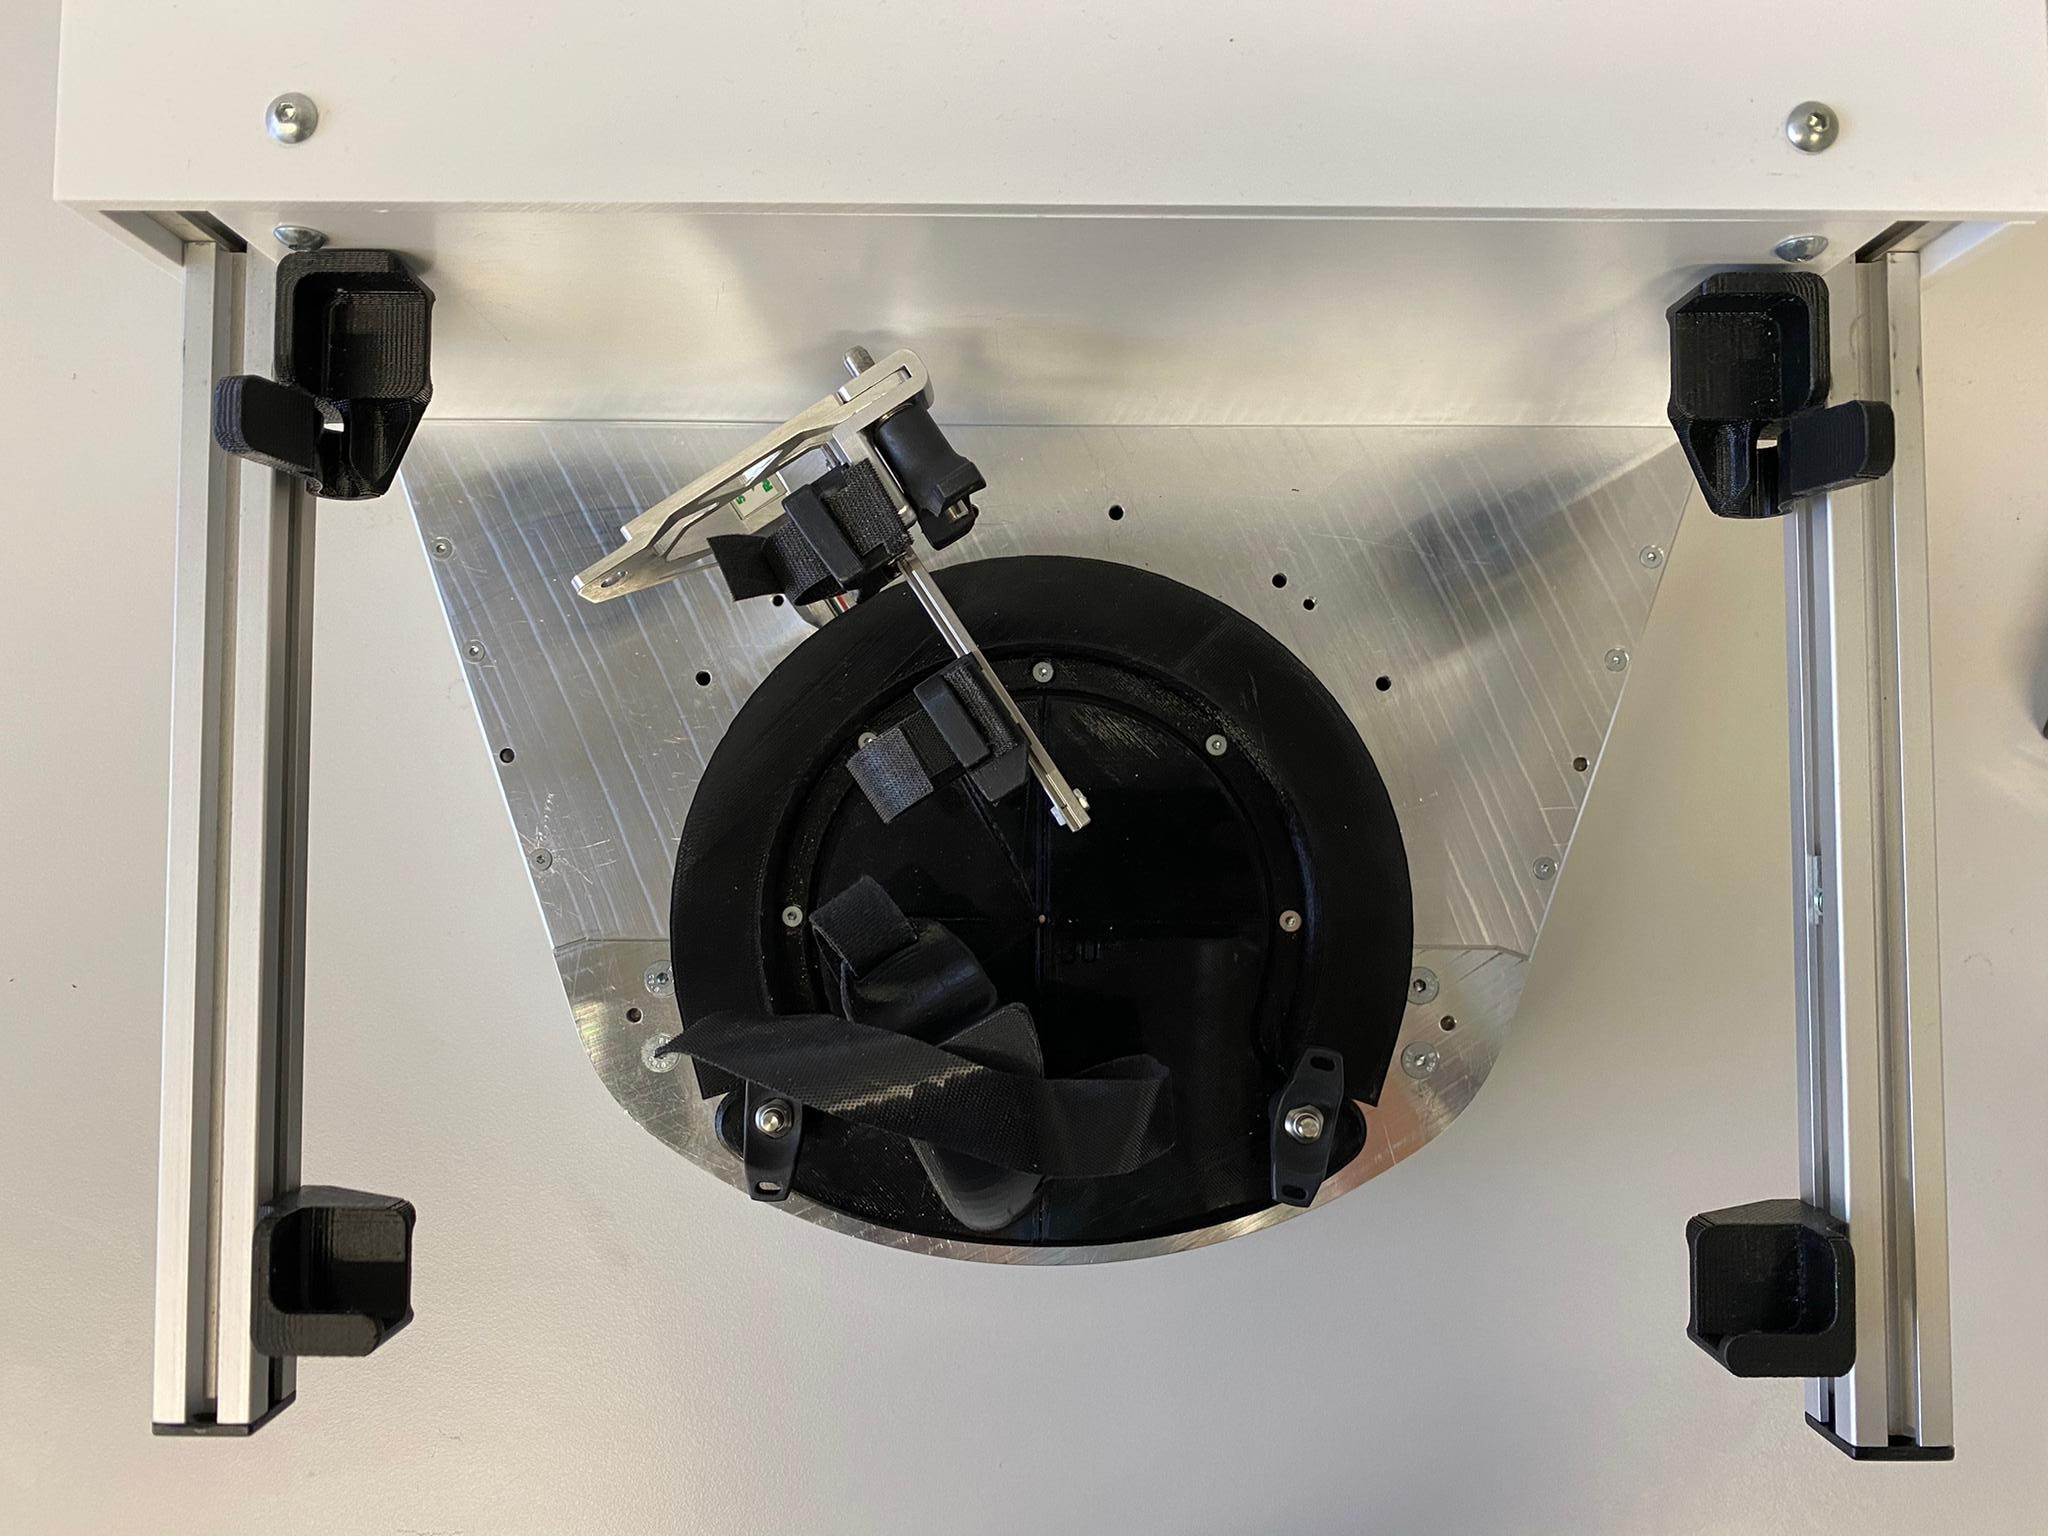
\includegraphics[width=\textwidth]{images/Hardware/rightside.jpeg}
\end{subfigure}\\
\vspace*{0.4cm}
\begin{subfigure}[b]{0.48\textwidth}
	\centering
	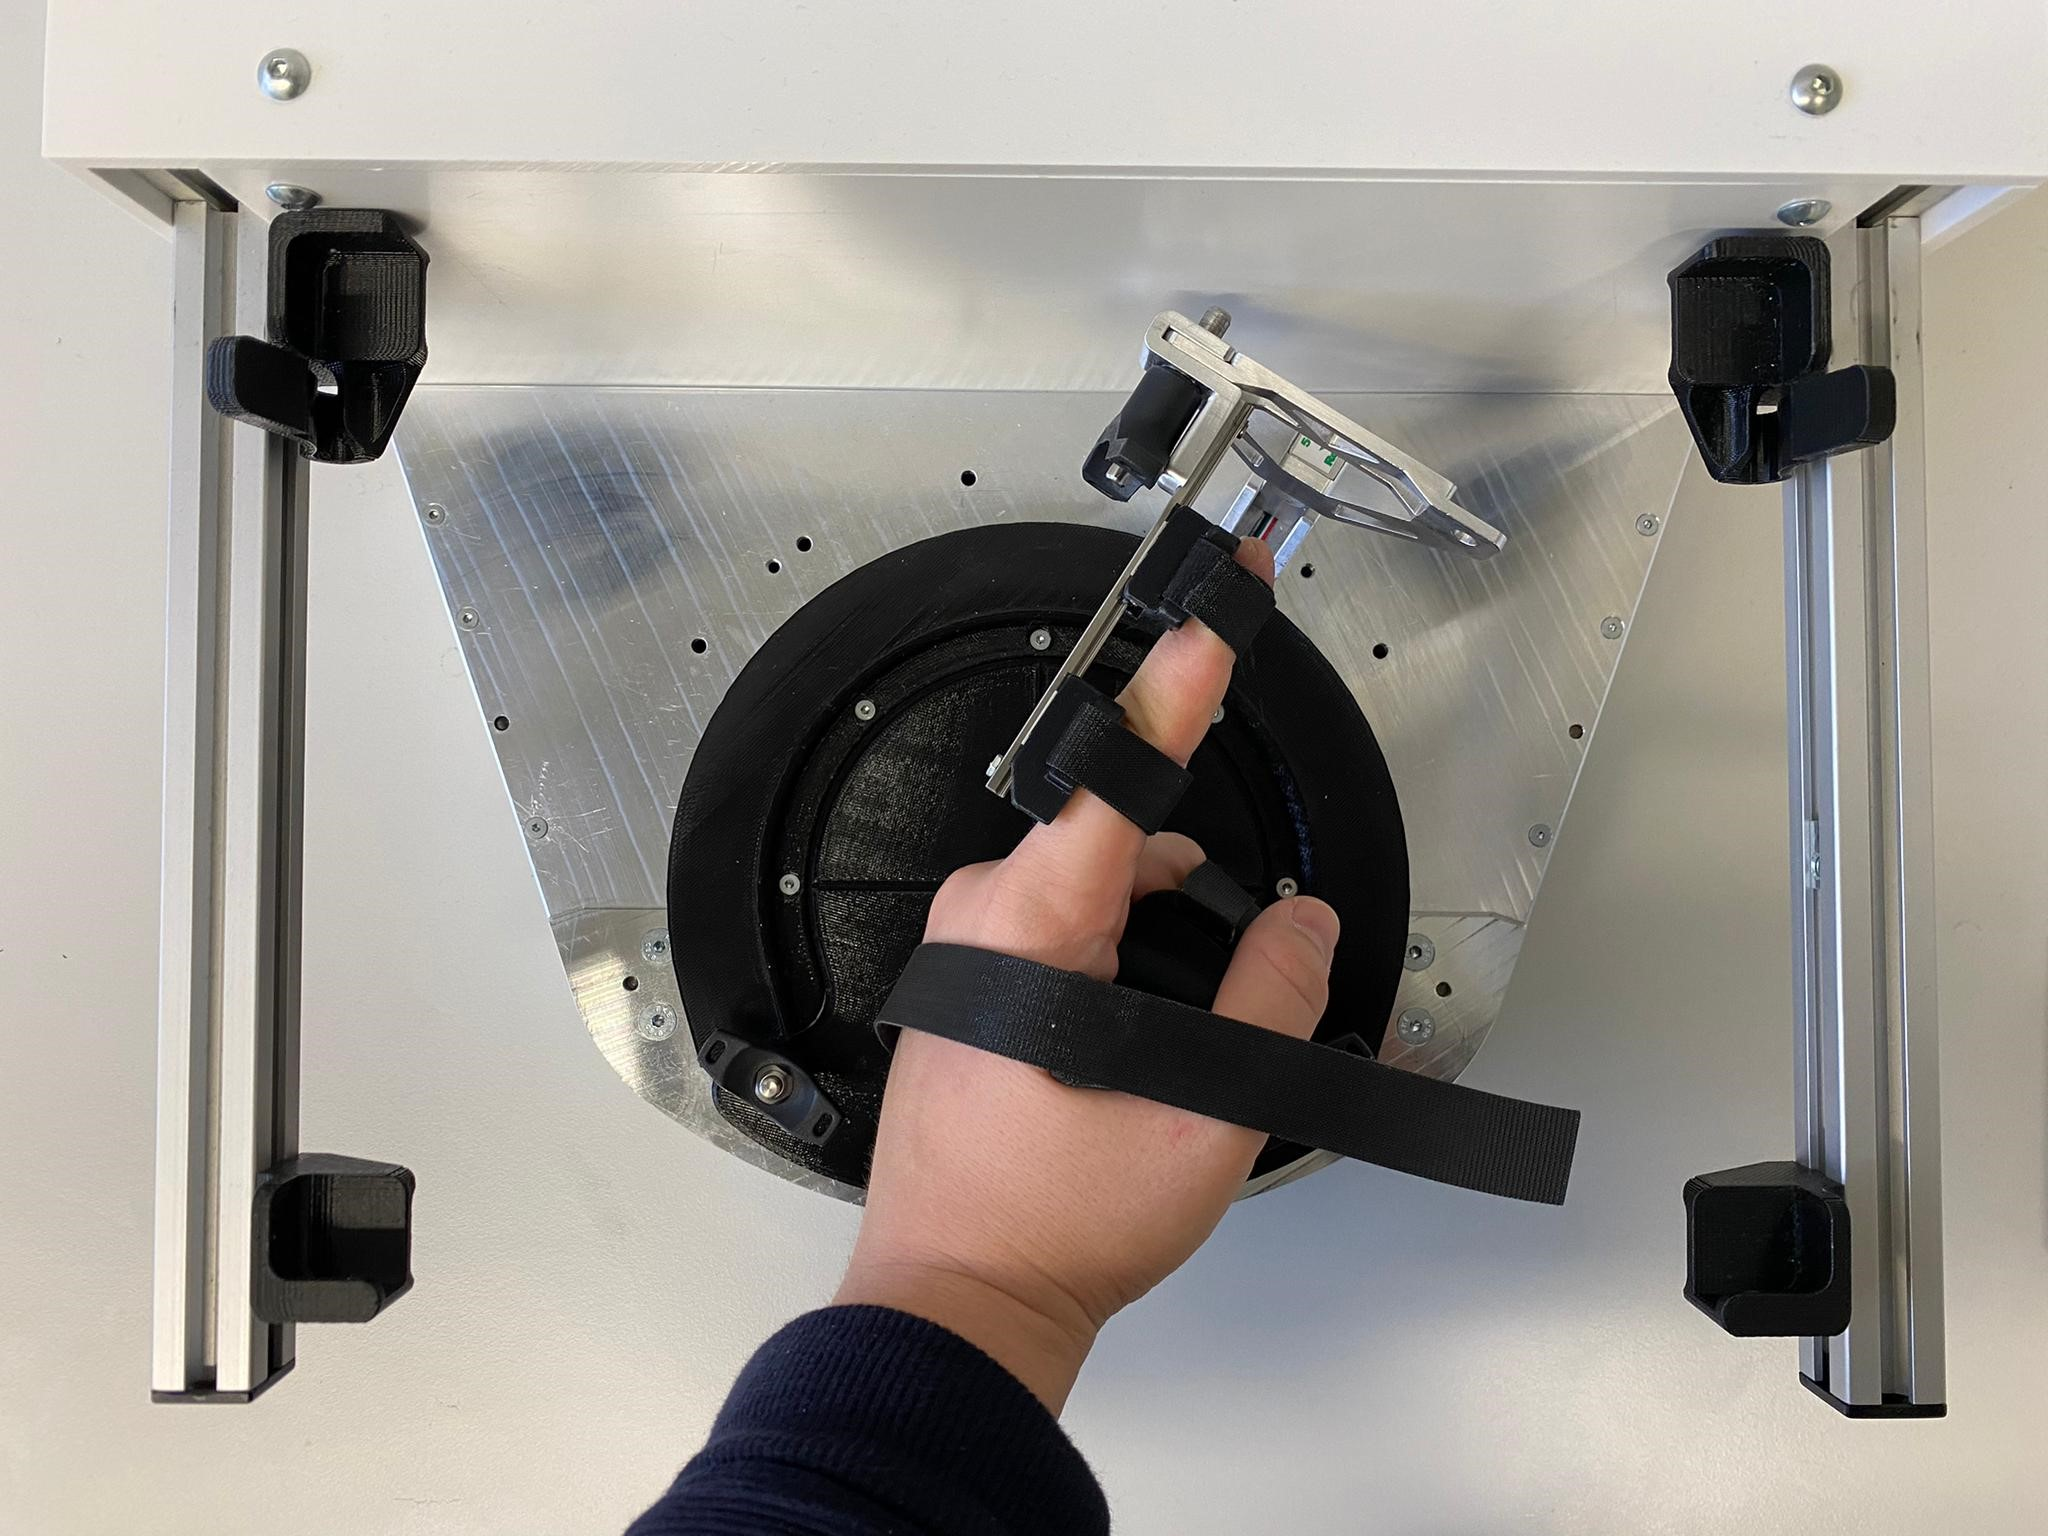
\includegraphics[width=\textwidth]{images/Hardware/hand1.jpeg}
\end{subfigure}
\hfill
\begin{subfigure}[b]{0.48\textwidth}
	\centering
	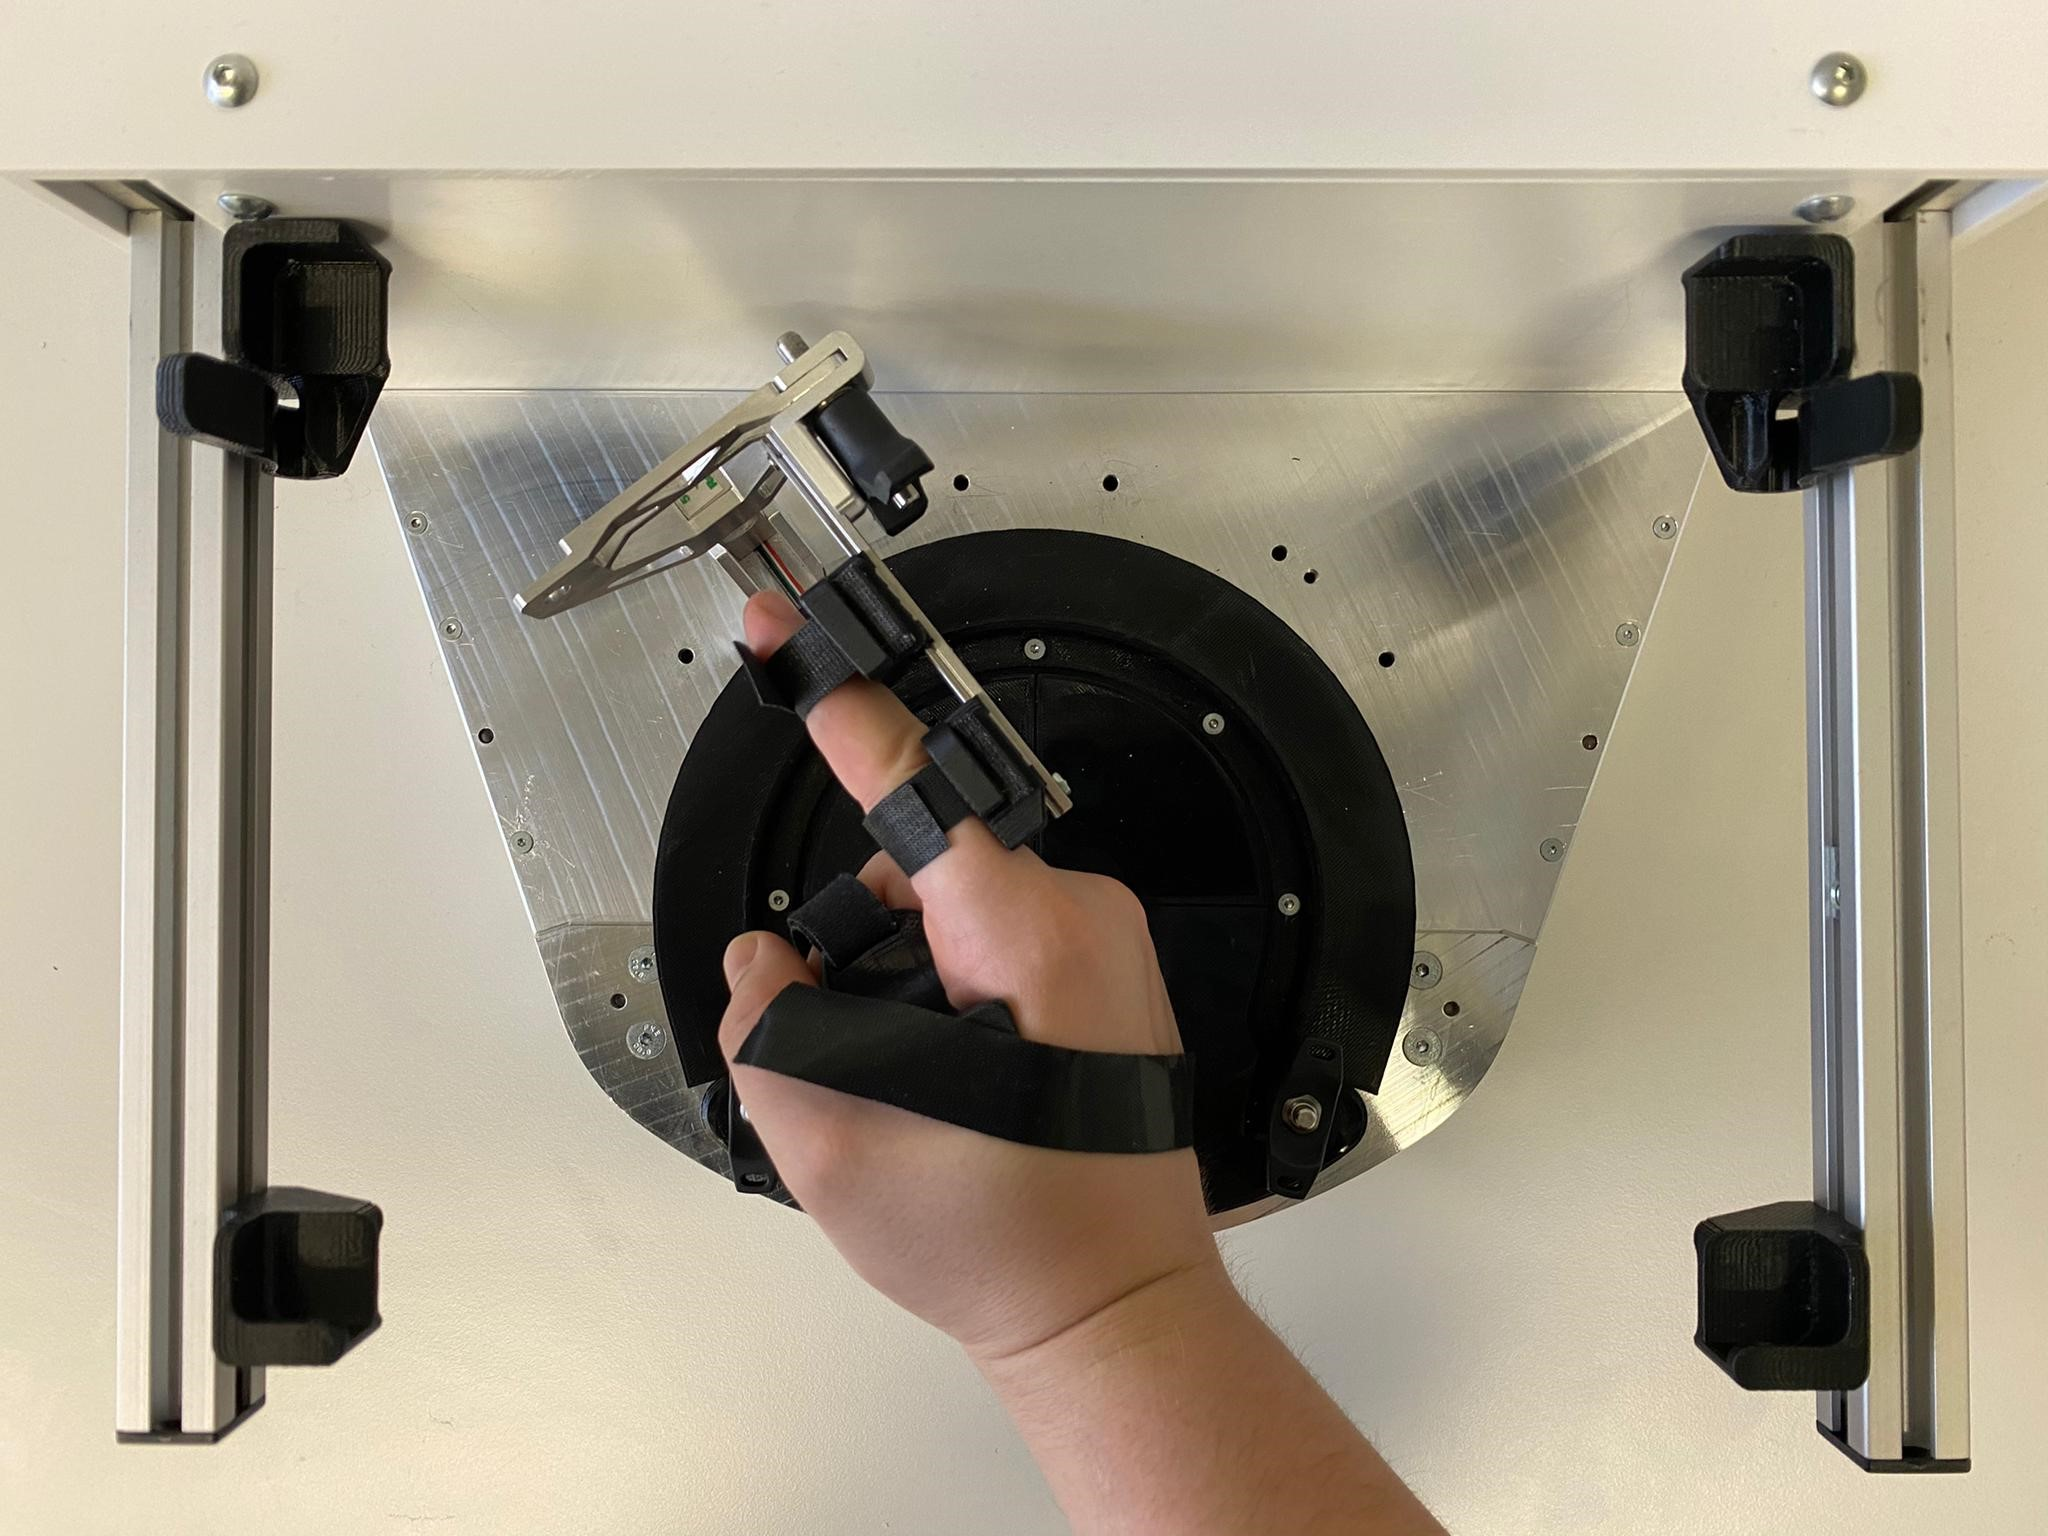
\includegraphics[width=\textwidth]{images/Hardware/hand2.jpeg}
\end{subfigure}
\caption{Placement of the handles and finger interface. The picture on the left demonstrates the setup for the left hand and the picture on the right the setup for the right hand.}
\label{fig:HandPlacement}
\end{figure}

\subsection{Placement of the Tablet}
Locate the tablet computer on the rails above the hand interface. Follow the steps indicated in Figure \ref{fig:tabletPlacement} to securely place and remove the tablet. 

\begin{figure}[h!]
\begin{center}
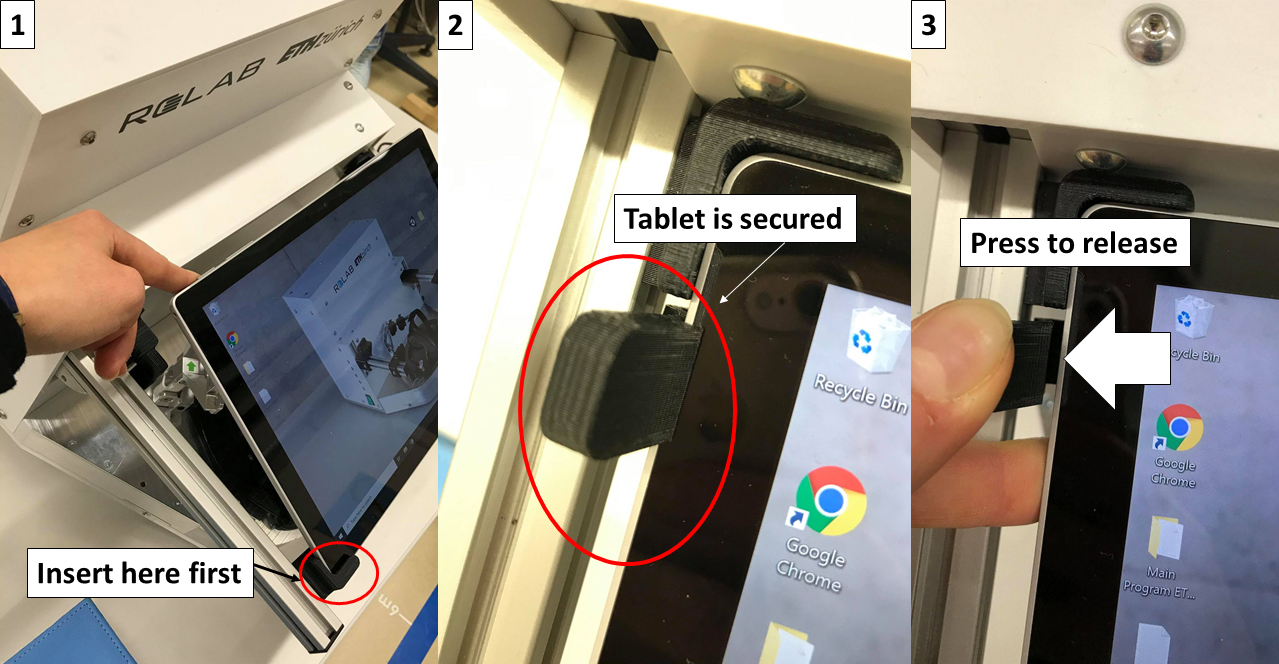
\includegraphics[width=\columnwidth]{images/Hardware/tabletPlacement.png}
\caption{Instructions on how to securely place and release the tablet on/from its rails.}
\label{fig:tabletPlacement}
\end{center}
\end{figure}

\subsection{Incline of the Device}
In order to avoid parallax error and ensure that participants are looking straight onto the tablet screen when performing the experiments, the robot needs to be placed at an inclined position. For that, we are using an incline plane (\#15 Table \ref{tab:parts}). Place the incline plane under the robot, as shown in Figure \ref{fig:incline}. During experiments, make sure that participants are sitting straight in front of the device with their elbow rested on an arm rest (Figure \ref{fig:incline}).

\begin{figure}[h!]
\centering
\begin{subfigure}[b]{0.4\textwidth}
	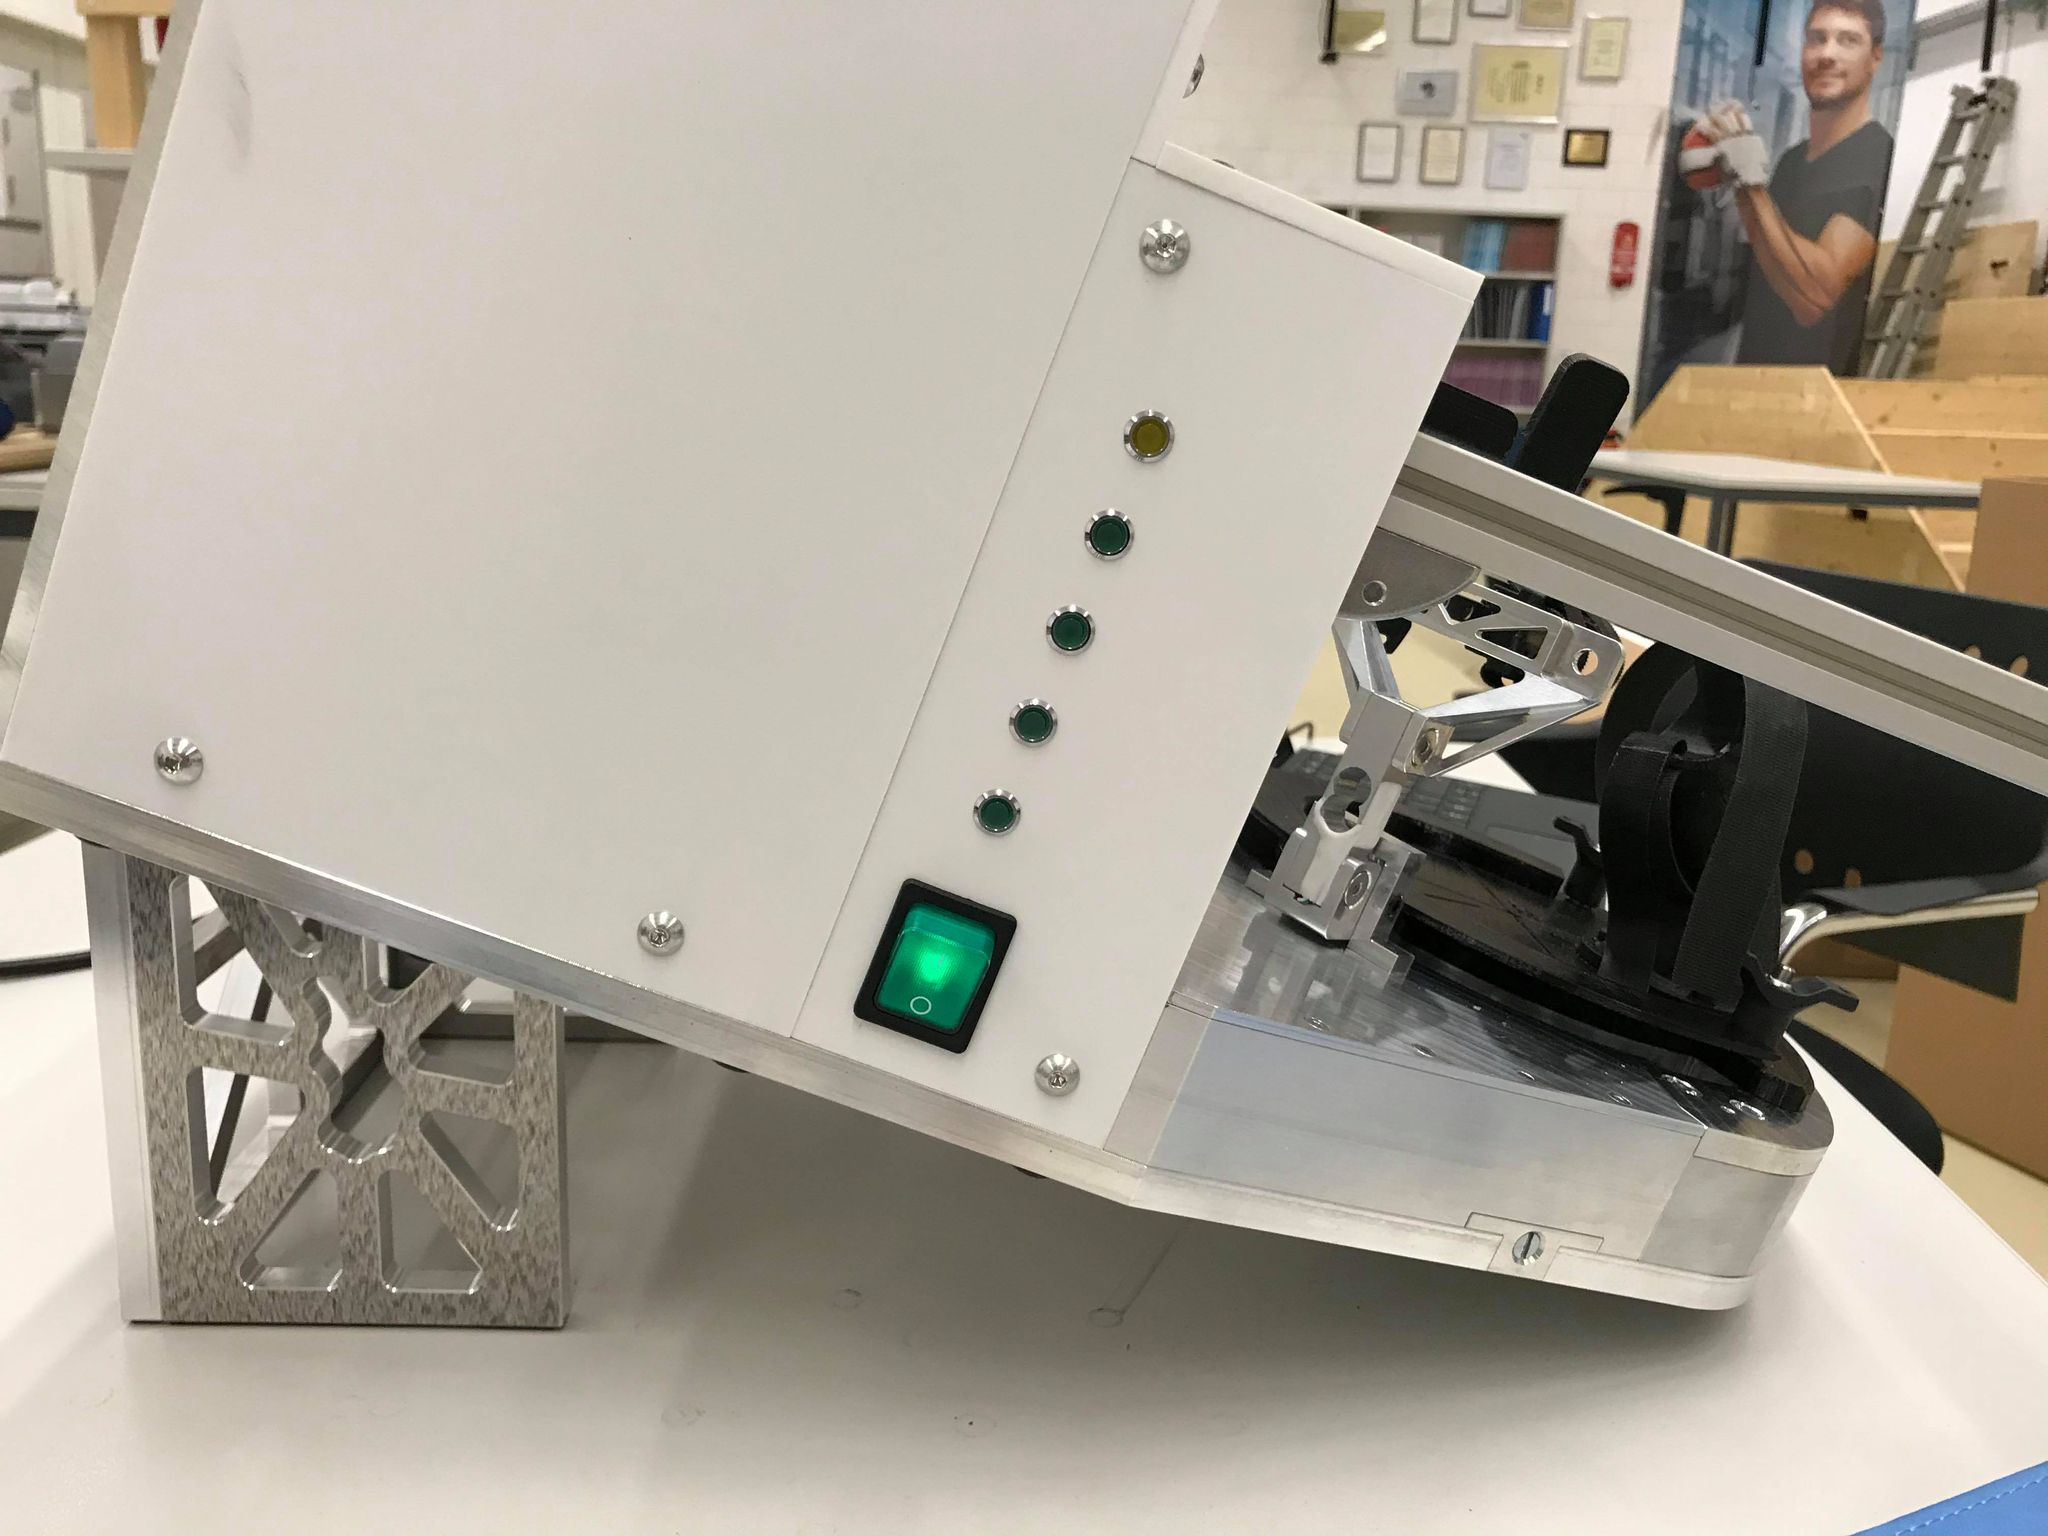
\includegraphics[height=4.6cm]{images/Hardware/Incline.jpg}
\end{subfigure}
\hfill
\begin{subfigure}[b]{0.58\textwidth}
	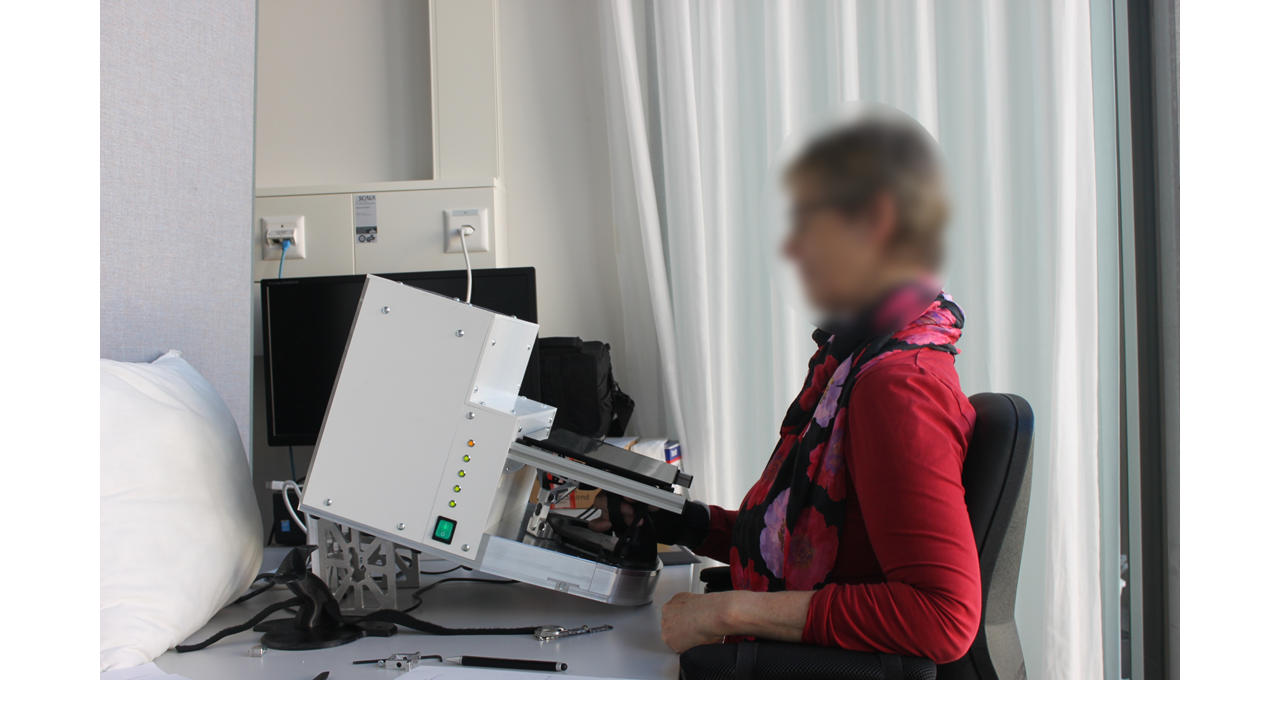
\includegraphics[height=4.6cm]{images/Subjects/SubjectsPosition.png}
\end{subfigure}
\caption{Incline plane placement and correct positioning of a study participant.}
\label{fig:incline}
\end{figure}

\subsection{How to Secure the Wrist for the Experiments}
It is necessary to ensure that there is no compensation from the wrist movements when performing the experiments (especially relevant for the range of motion task to avoid hyperextension due to the wrist rotation). First, locate a protection on subject’s wrist in a form of Tricofix sleeve. Then, place the wrist splint and wrap it around with the Leukotape bandage to secure (Figure \ref{fig:WristSplint}). Throw away the sleeve and the piece of bandage after use and disinfect the wrist splint (reusable). The wrist splint is suitable for both hands. 

\begin{figure}[h!]
\begin{center}
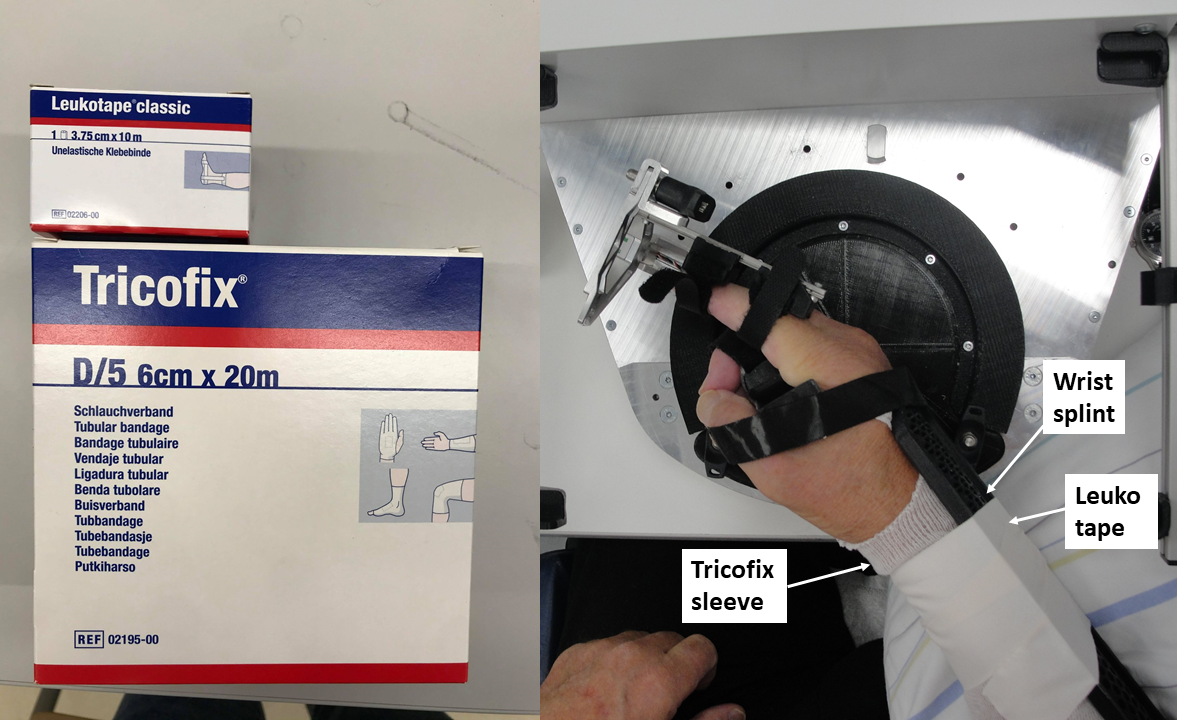
\includegraphics[width=\columnwidth]{images/Hardware/WristSplint.png}
\caption{How to secure the wrist for experiments. This is especially important for the range of motion task to avoid hyperextension due to wrist rotation.}
\label{fig:WristSplint}
\end{center}
\end{figure}

\subsection{Calibration and Switching on}
\subsubsection*{Calibration}
The robot needs to be calibrated every time it is switched on. Once it is switched on, there is no need to recalibrate it. Ensure the robot is switched on only when you are using it and that you don’t leave it switched on overnight. \\

In order to calibrate the robot, place the end-effector lock (\#16 Table \ref{tab:parts}) so that it locks the end-effector in the middle position (as shown in Figure 9). \\

This calibration process needs to be performed when you switch the device on. Wait a couple of seconds with the metal element inserted in the correct place until all LEDs are switched on and you hear a clicking sound (this is when calibration happens). After this, you can remove the end-effector lock and move the end-effector freely. The end-effector lock is used again in the Force Task (see instructions for individual assessments in Section \ref{sec:AssessmentTasks}). \\

Note: when you first unpack the device, the end-effector lock is already in place (protection for transportation). The end-effector lock was tightened for transportation purposes. To loosen it, use Allen key (\#14 Table \ref{tab:parts}) by turning the screw on the side of the metal piece. 

\begin{figure}[h!]
\begin{center}
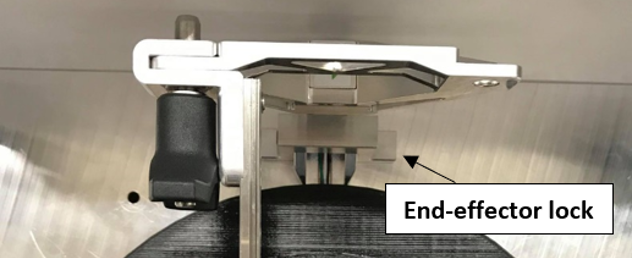
\includegraphics[width=0.7\columnwidth]{images/Hardware/Calibration.png}
\caption{Calibration of the ETH MIKE using the end-effector lock by positioning the end-effector in the centre. Ensure the end-effector is in this position every time you switch on the robot. }
\label{fig:Calibration}
\end{center}
\end{figure}

\subsubsection*{LEDs}
When the robot is switched off, all LEDs are also off (Figure \ref{fig:LED}A). Once the robot is switched on and the emergency button is released, 4 out of 5 LEDs will be turned on (Figure \ref{fig:LED}C). Then, after a few seconds (this is when the end-effector lock needs to be correctly inserted as in Figure \ref{fig:Calibration}), all LEDs will be switched on (Figure \ref{fig:LED}D). If the emergency button is pressed, not all LEDs will be turned on (Figure \ref{fig:LED}B). Ensure the emergency button is released and all LEDs are switched on when using the robot for experiments. 

\begin{figure}[h!]
\begin{center}
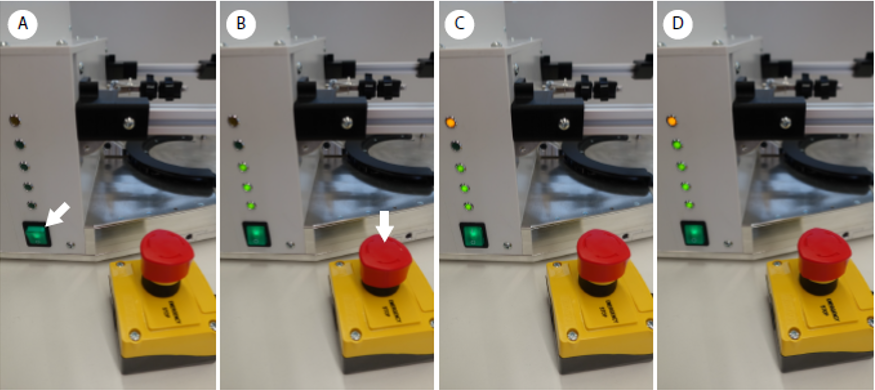
\includegraphics[width=\columnwidth]{images/Hardware/LEDs.png}
\caption{States of the LEDs on the side of the device.}
\label{fig:LED}
\end{center}
\end{figure}

\newpage
\section{Software}
\subsection{ETH MIKE Program}
To start using the ETH MIKE robot software, first switch on the tablet (button on the top). Then, log in to the user “ETH-MIKE-x” with the password “admin”. \\

On the desktop, find the following: “ETH Mike – Shortcut” and “ETH MIKE xxx” folder. The first one is the main software and the other is the folder where all data is stored. 

\begin{figure}[h!]
\begin{center}
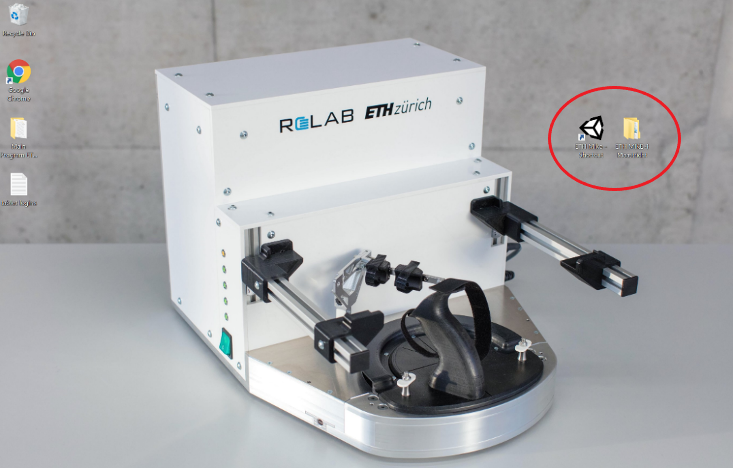
\includegraphics[width=\columnwidth]{images/Hardware/Desktop.png}
\caption{The tablet desktop with indicated files/folders of importance.}
\label{fig:desktop}
\end{center}
\end{figure}

\subsection{Login}
The initial view of the “ETH Mike – Shortcut” application is shown in Figure \ref{fig:LoginView}. First click on the person icon to create a new subject account. A Subject ID will be generated (Figure \ref{fig:Registration}). Write down that ID as you will need it to identify stored data. After you create a new login, click “New session” to start the assessments. In case you log-out during an assessment session and would like to resume, click “Resume last session”. 

\begin{figure}[h!]
\begin{center}
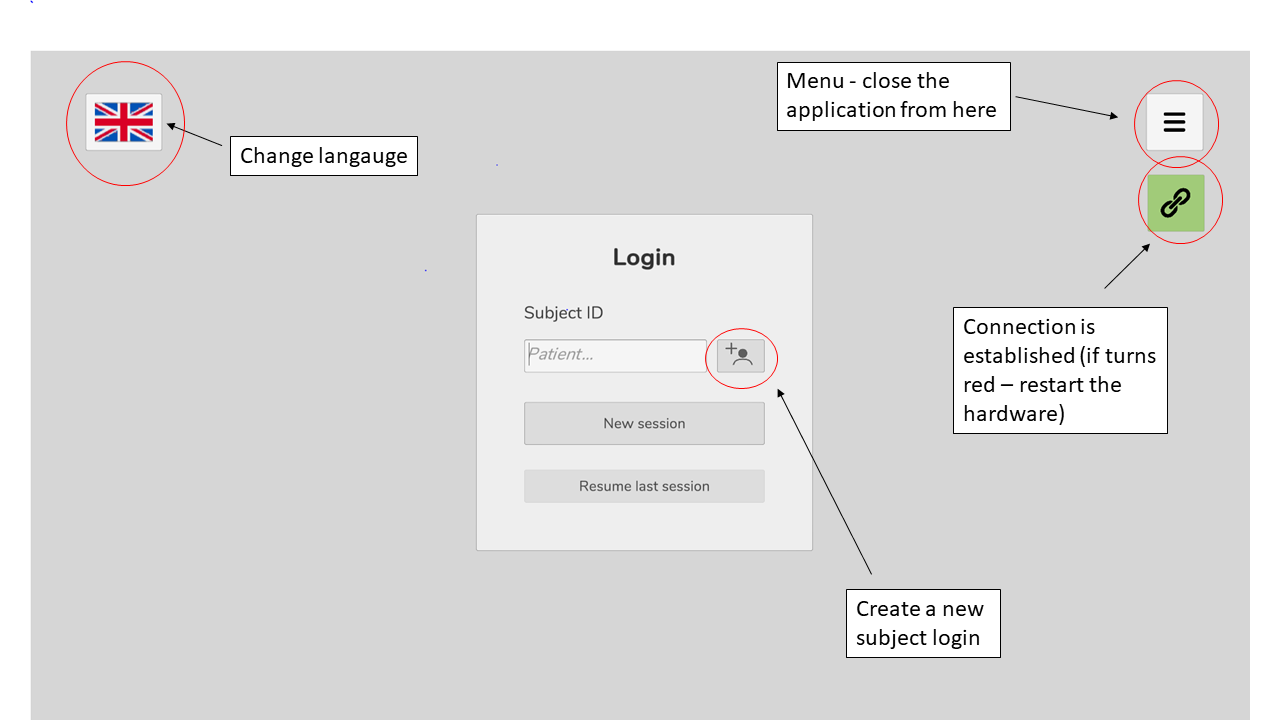
\includegraphics[width=\columnwidth]{images/TabletScreenshots/LoginView.png}
\caption{Login view of the ETH MIKE software application.}
\label{fig:LoginView}
\end{center}
\end{figure}

\begin{figure}[h!]
\begin{center}
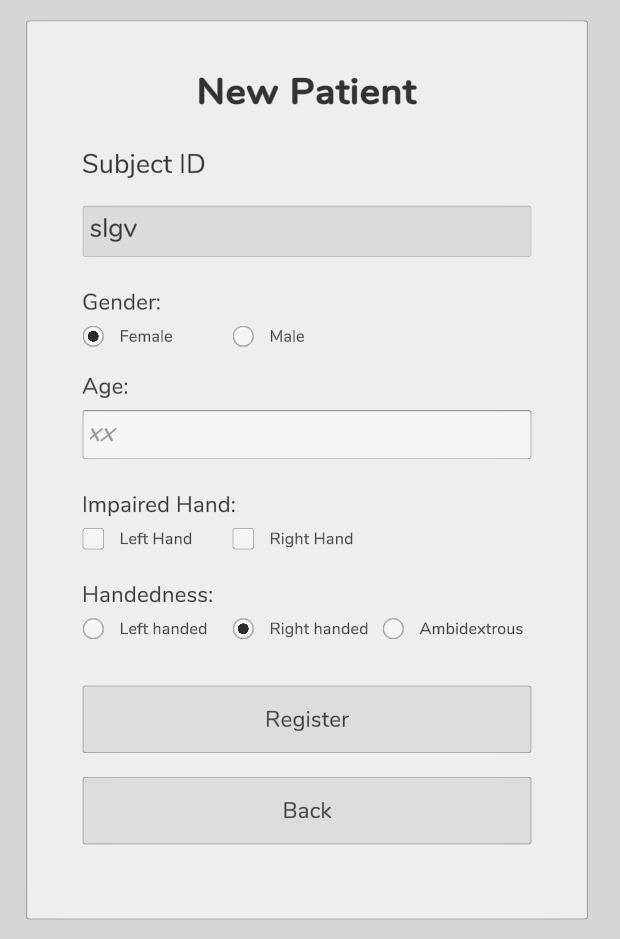
\includegraphics[width=0.48\columnwidth]{images/Assessments/NewSubject.png}
\caption{Window for creating as new subject. Subject ID is automatically generated, under which all data for this subject will be stored – write down this subject ID to be able to identify your files later.}
\label{fig:Registration}
\end{center}
\end{figure}

\newpage
\phantom{blabla}
\newpage
\section{Assessment Tasks}
\label{sec:AssessmentTasks}
For a video explanation of all tasks, watch \href{https://www.youtube.com/watch?v=jmWdwJ00onU&t=3s&ab_channel=RELABETHZ}{this video}. 

\subsection{Task Selection Menu}
Task selection menu is shown in Figure \ref{fig:TaskSelectionMenu}. It allows you to select the hand (use the slider to switch between right and left hand) and the task you want to perform. Question marks contain explanation of the procedure of each task, as well as a possibility to conduct practice trials. A task completion during a session is indicated by a tick next to it, see Force task in Figure \ref{fig:TaskSelectionMenu}.

\begin{figure}[h!]
\begin{center}
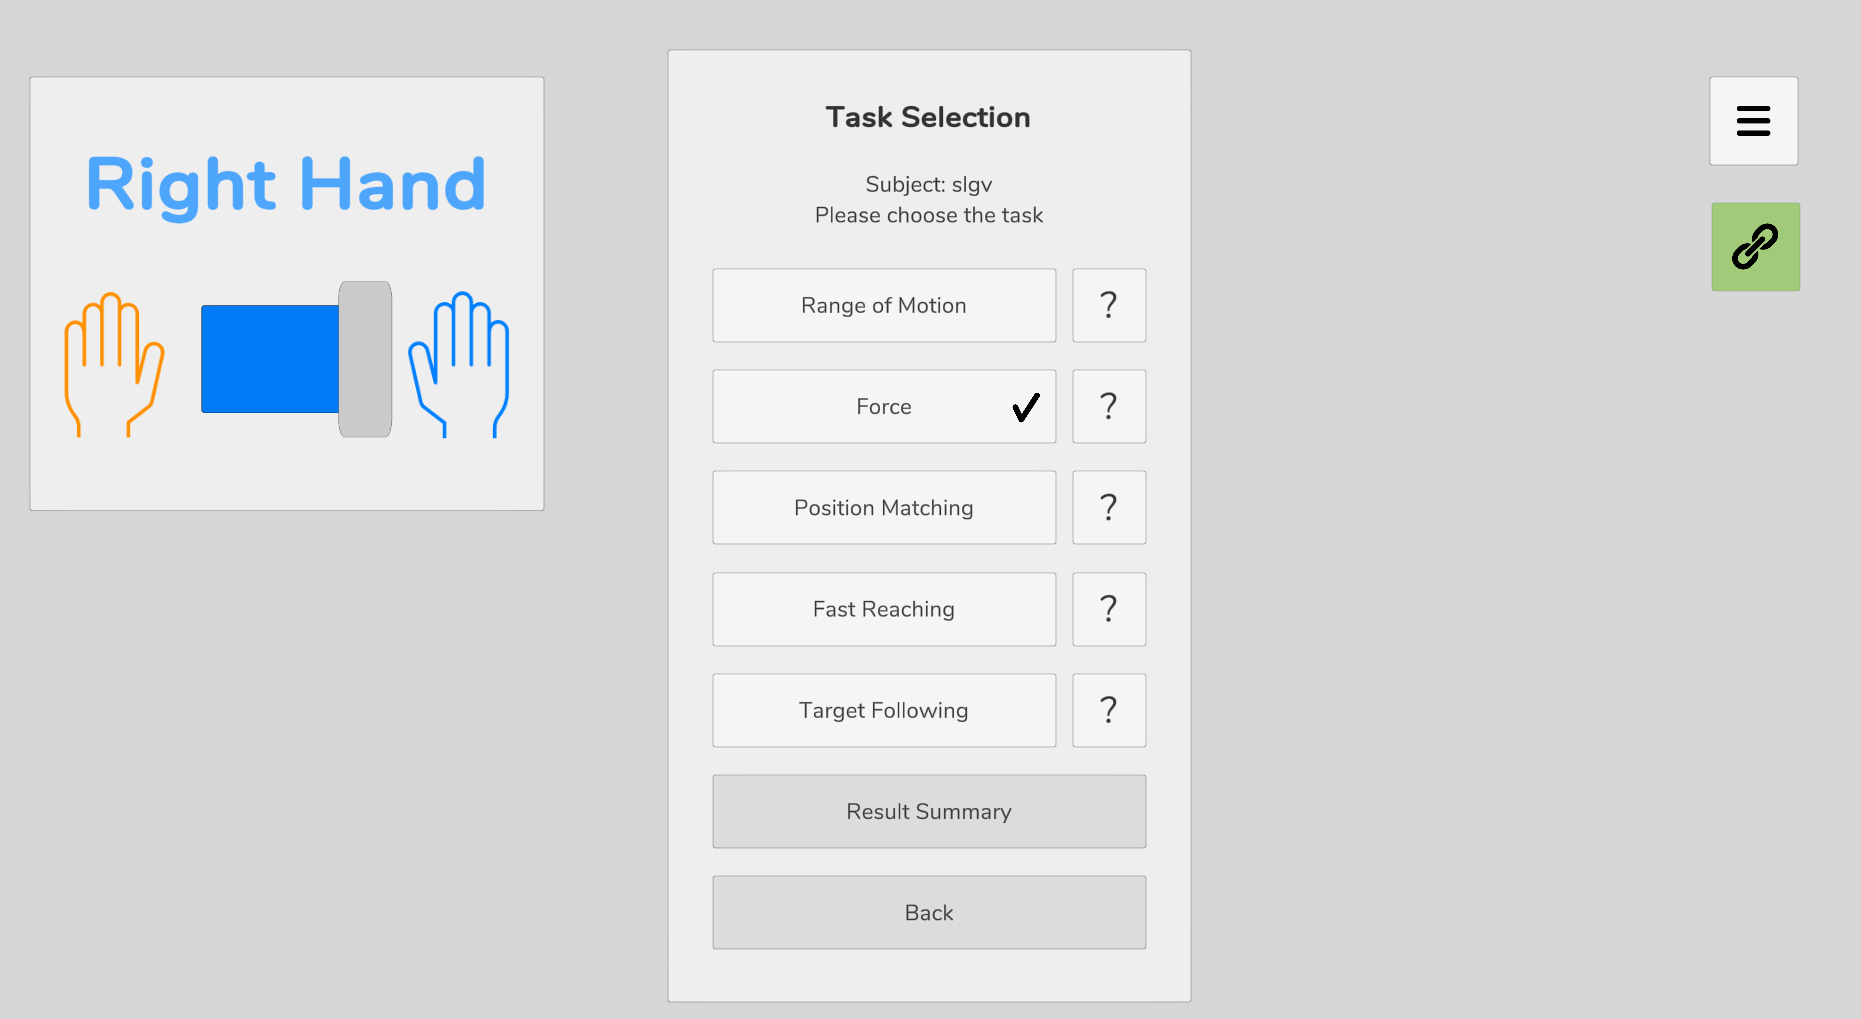
\includegraphics[width=\columnwidth]{images/Assessments/TaskSelectionMenu.png}
\caption{Assessment task selection menu.}
\label{fig:TaskSelectionMenu}
\end{center}
\end{figure}

\subsection{Range of Motion (motor impairments)}
\subsubsection*{Active Range of Motion}
First flex (bend) your finger as far as possible and then extend (stretch) it. The blue needle indicates your finger position. Before each trail the finger is first automatically moved to the starting position by the robot (\emph{Get ready}). Once you have performed the movement, click \emph{Finish} to proceed to the next trial. There are 3 trials.  

\subsubsection*{Passive Range of Motion}
The tablet needs to be removed for this part of the experiment to allow the experimenter to access the subject’s finger. The experimenter moves the participant’s finger to maximum flexion and then maximum extension. The finger is automatically moved to the starting position by the robot before each trial (\emph{Get ready}). Once you have performed the movement, click \emph{Finish} to proceed to the next trial. The participant needs to relax his/her finger throughout the trial. There are 3 trials.

\subsubsection*{Automatic Passive Movement}
The tablet remains removed for this part of the experiment. Participant’s finger will be automatically moved 3 times within the passive range of motion. The participant needs to relax his/her finger. 

\begin{figure}[h!]
\begin{center}
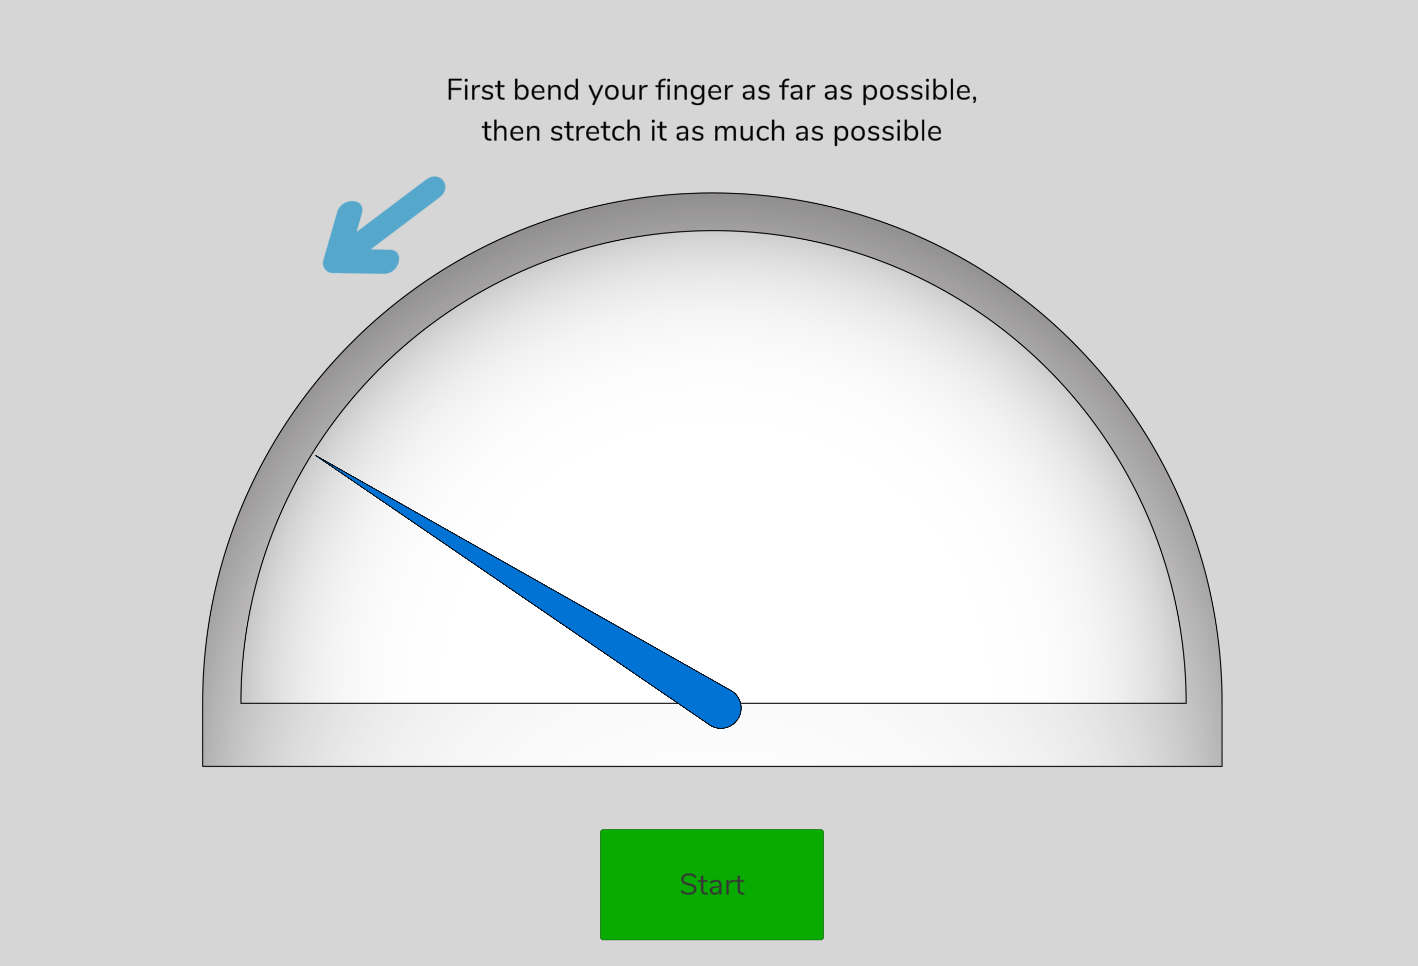
\includegraphics[width=\columnwidth]{images/Assessments/RangeOfMotion.png}
\caption{Instructions of the active range of motion task. }
\label{fig:ROM}
\end{center}
\end{figure}

\subsection{Force (motor impairments)}
The end-effector lock needs to be inserted for this task. Remove the tablet and insert the end effector lock as demonstrated in Figure \ref{fig:EndeffoctorLock} (at 45 degrees). After securing the end-effector, place the tablet above the hand on the designated rails again. \\

The instruction of this task is to generate maximum fingertip force, first in flexion, then in extension. When prompted on the screen (as shown in Figure \ref{fig:ForceTask}), flex (bend) you finger with as much force as possible. This is repeated 3 times, followed by 3 times extension (stretch). There is a 3 seconds preparation phase before the 3 seconds force generation phase. \\

Remove the end-effector lock after completion of the task. 

\begin{figure}[h!]
\centering
\begin{subfigure}[b]{0.48\textwidth}
	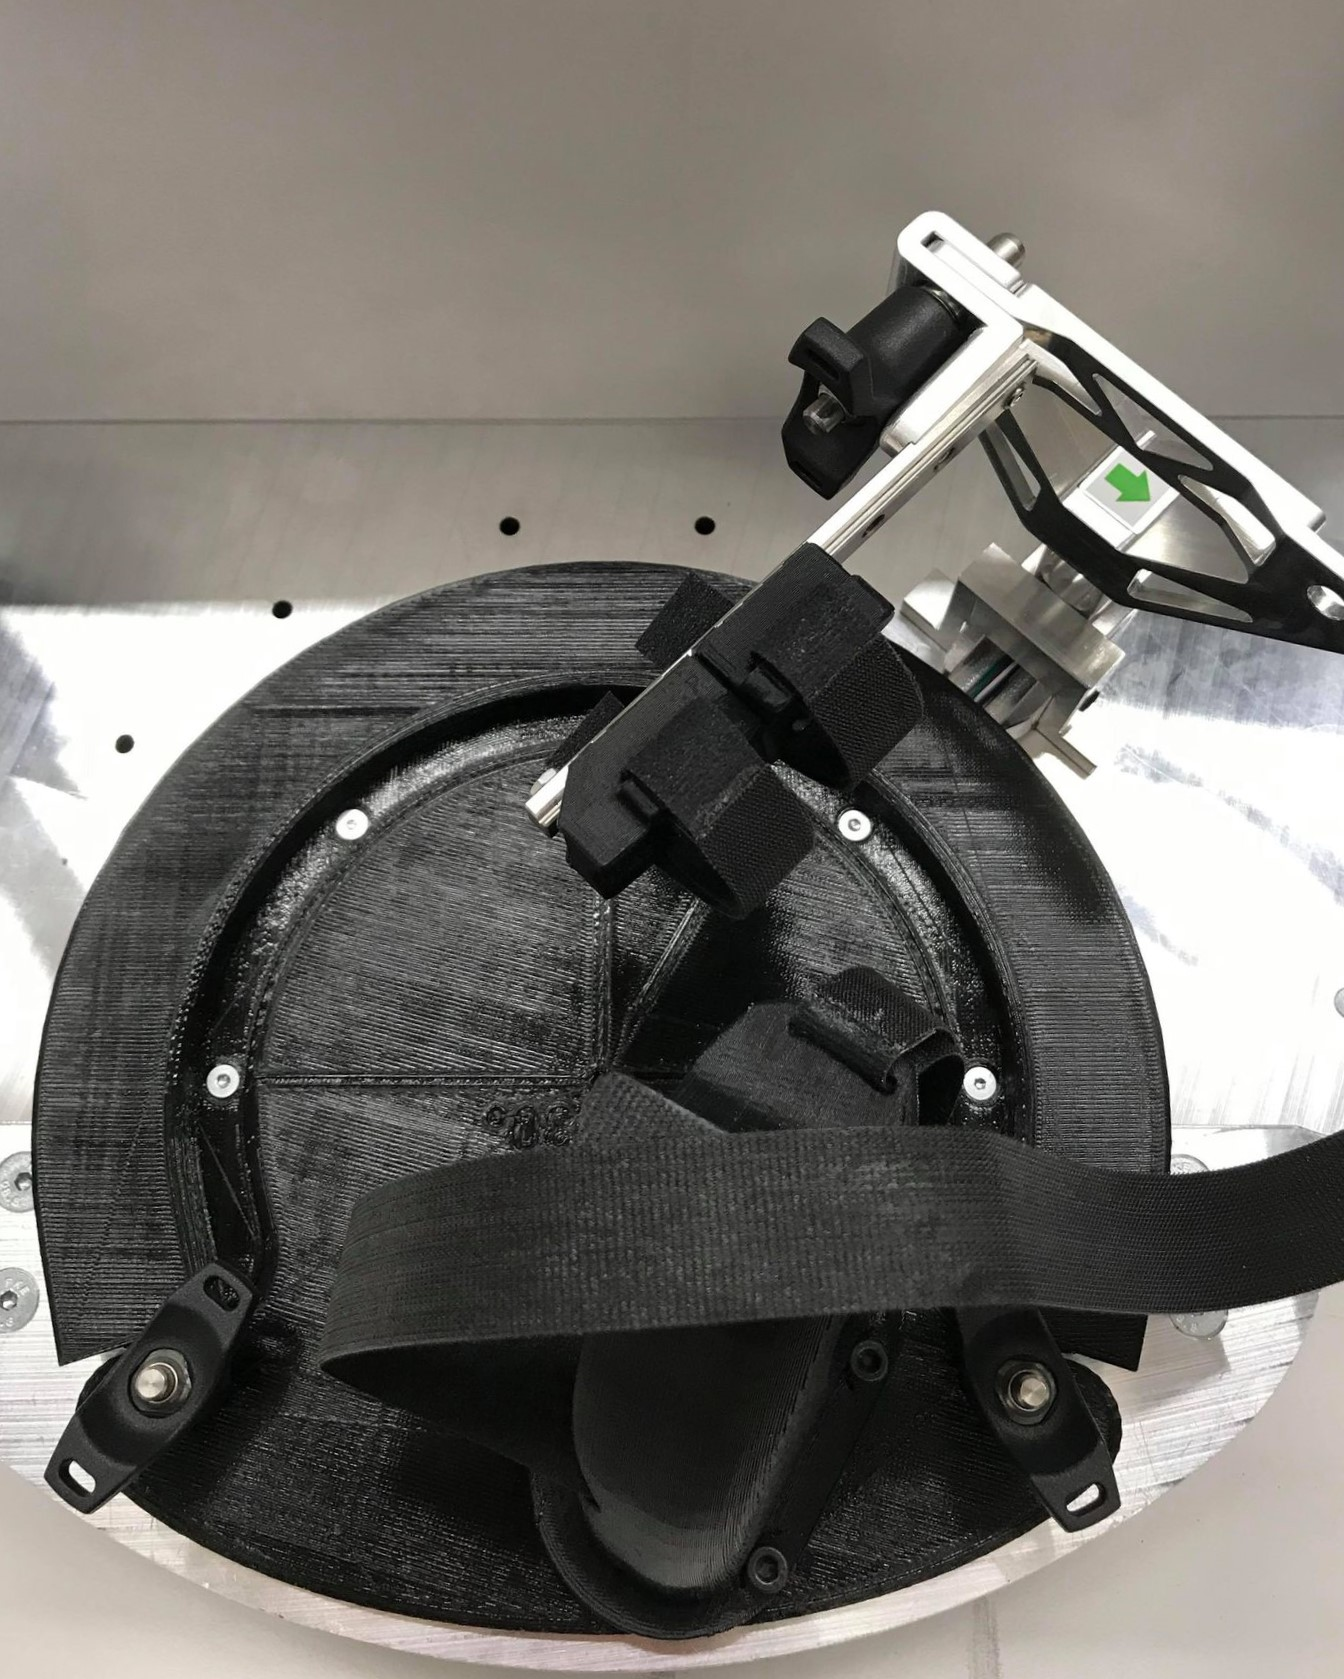
\includegraphics[width=\textwidth]{images/Hardware/ForceTask1.jpg}
\end{subfigure}
\hfill
\begin{subfigure}[b]{0.48\textwidth}
	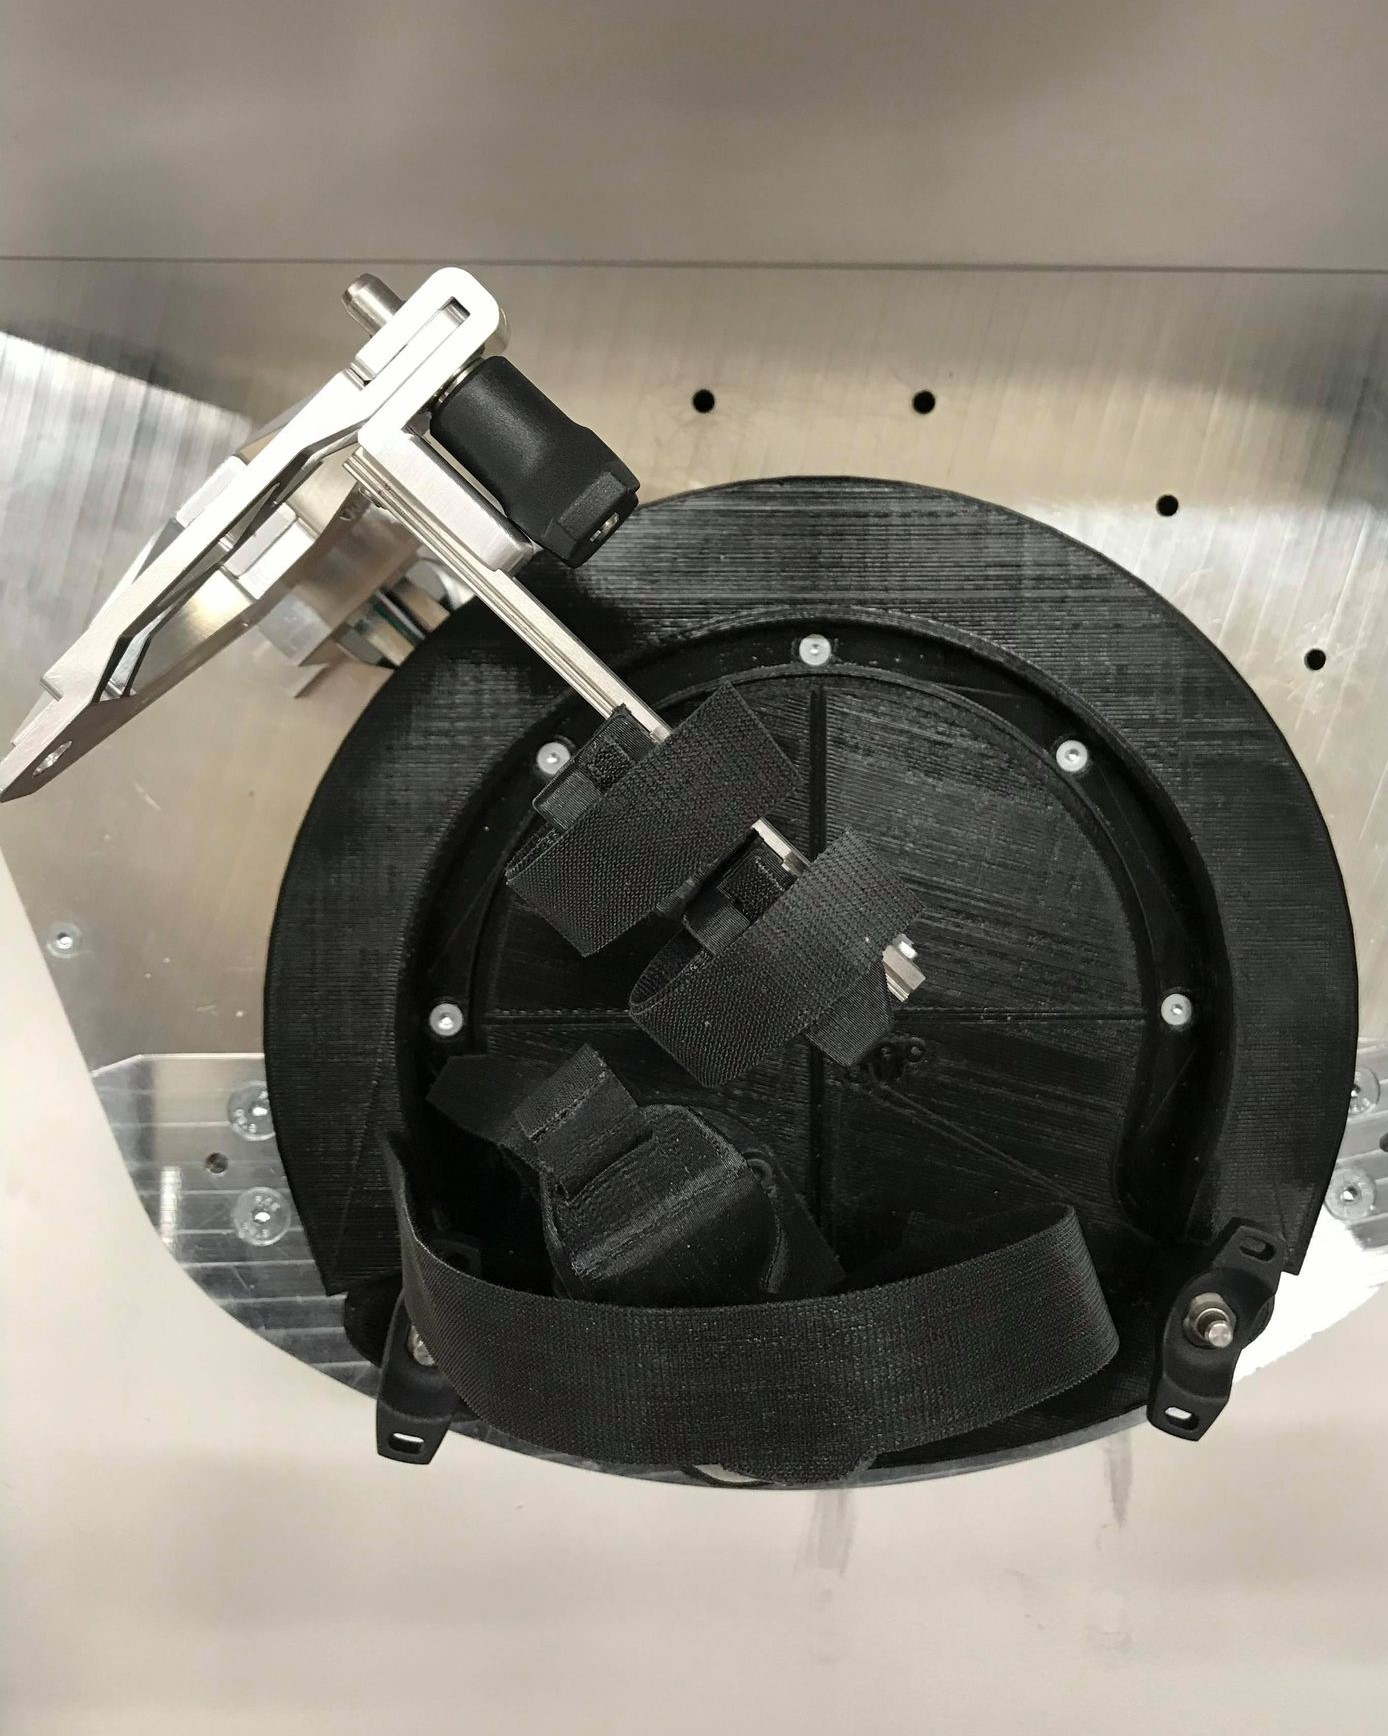
\includegraphics[width=\textwidth]{images/Hardware/ForceTask2.jpg}
\end{subfigure}
\caption{Location of the end-effector lock for the left hand (left side) and the right hand (right side) for the maximum fingertip force generation task.}
\label{fig:EndeffoctorLock}
\end{figure}

\begin{figure}[h!]
\begin{center}
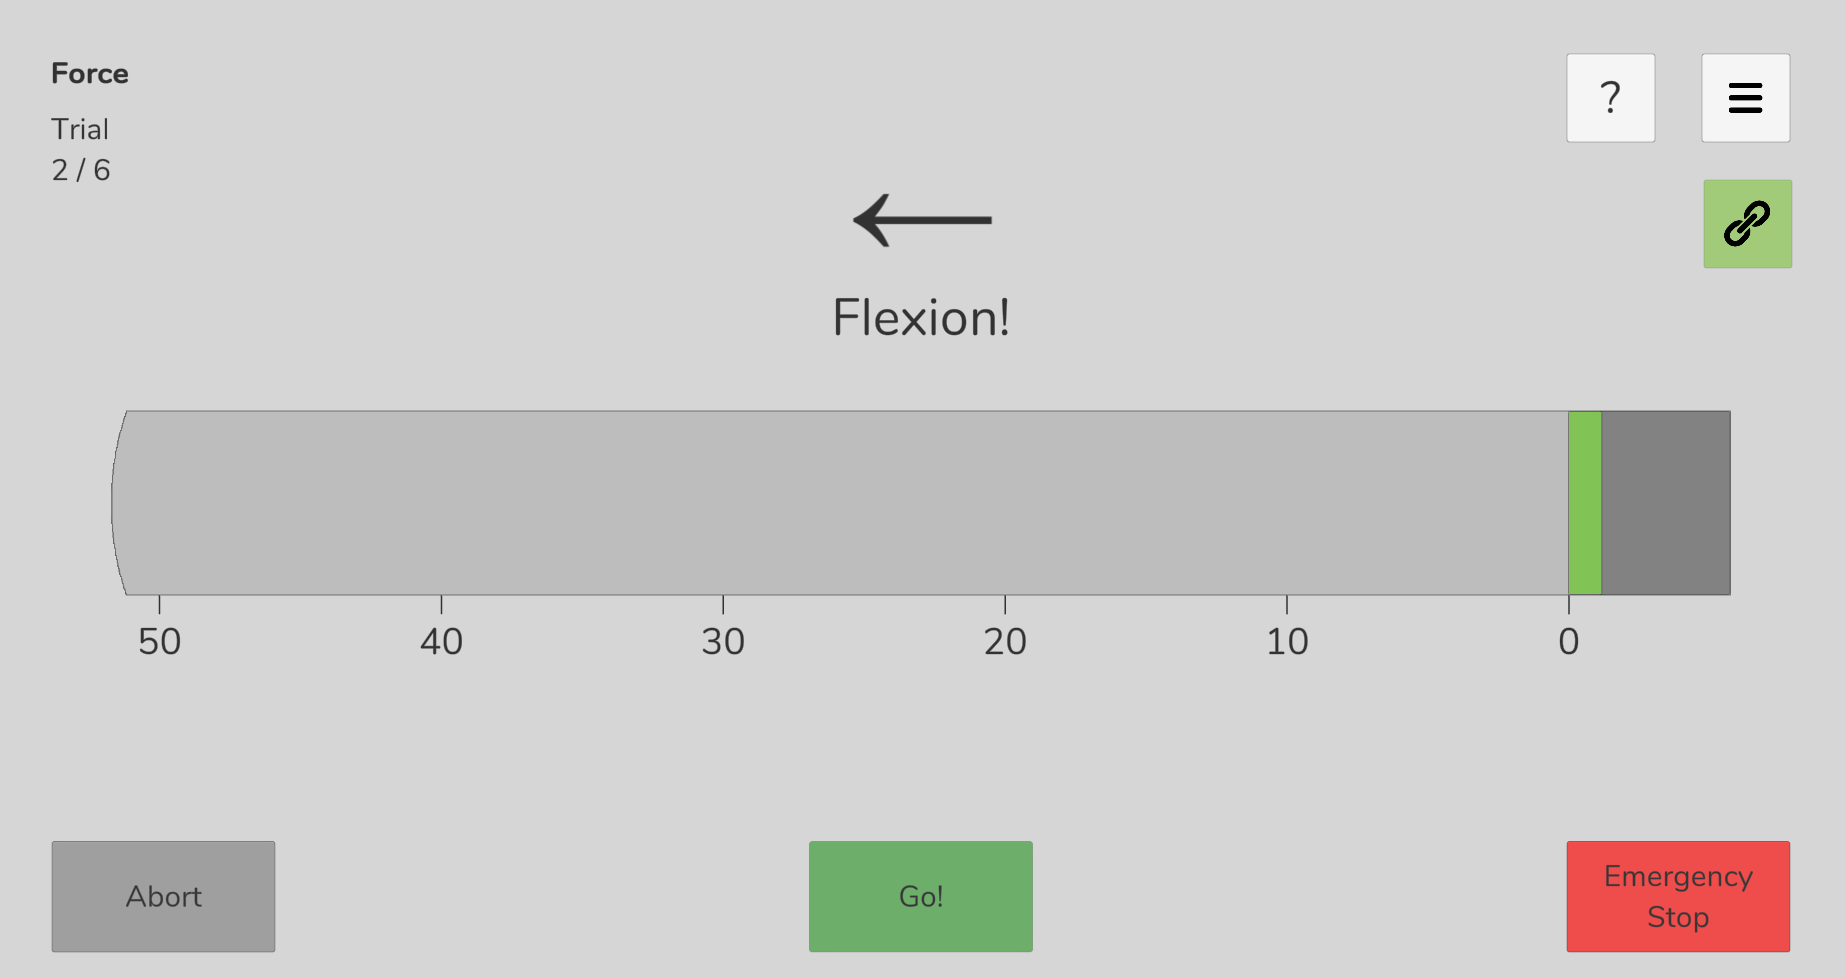
\includegraphics[width=0.7\columnwidth]{images/Assessments/Force.png}
\caption{Interface of the Force Task indicating to bend the finger as strong as possible.}
\label{fig:ForceTask}
\end{center}
\end{figure}

\subsection{Position Matching (proprioception impairments)}
The objective of this task is to measure the finger position perceived by the subject without visual feedback (due to the placement of the tablet), thereby relying on proprioception.\\

The robot first moves the finger to a starting position (indicated in red) and then immediately to a new position. Drag the green gauge needle to indicate the currently perceived finger position (Figure \ref{fig:PositionMatching}). Tap \emph{Validate} to confirm your selection. In case the participant is unable to indicate on the screen by him/herself with the other hand, the experimenter moves the gauge needle for him/her by asking “is the finger above/below” and dragging the needle until the participant says stop. There are 11 repetitions.\\

This task is normally the most challenging to understand, therefore it is recommended to perform practice round before, where visual feedback is provided for 3 trials. 

\begin{figure}[h!]
\centering
\begin{subfigure}[b]{0.48\textwidth}
	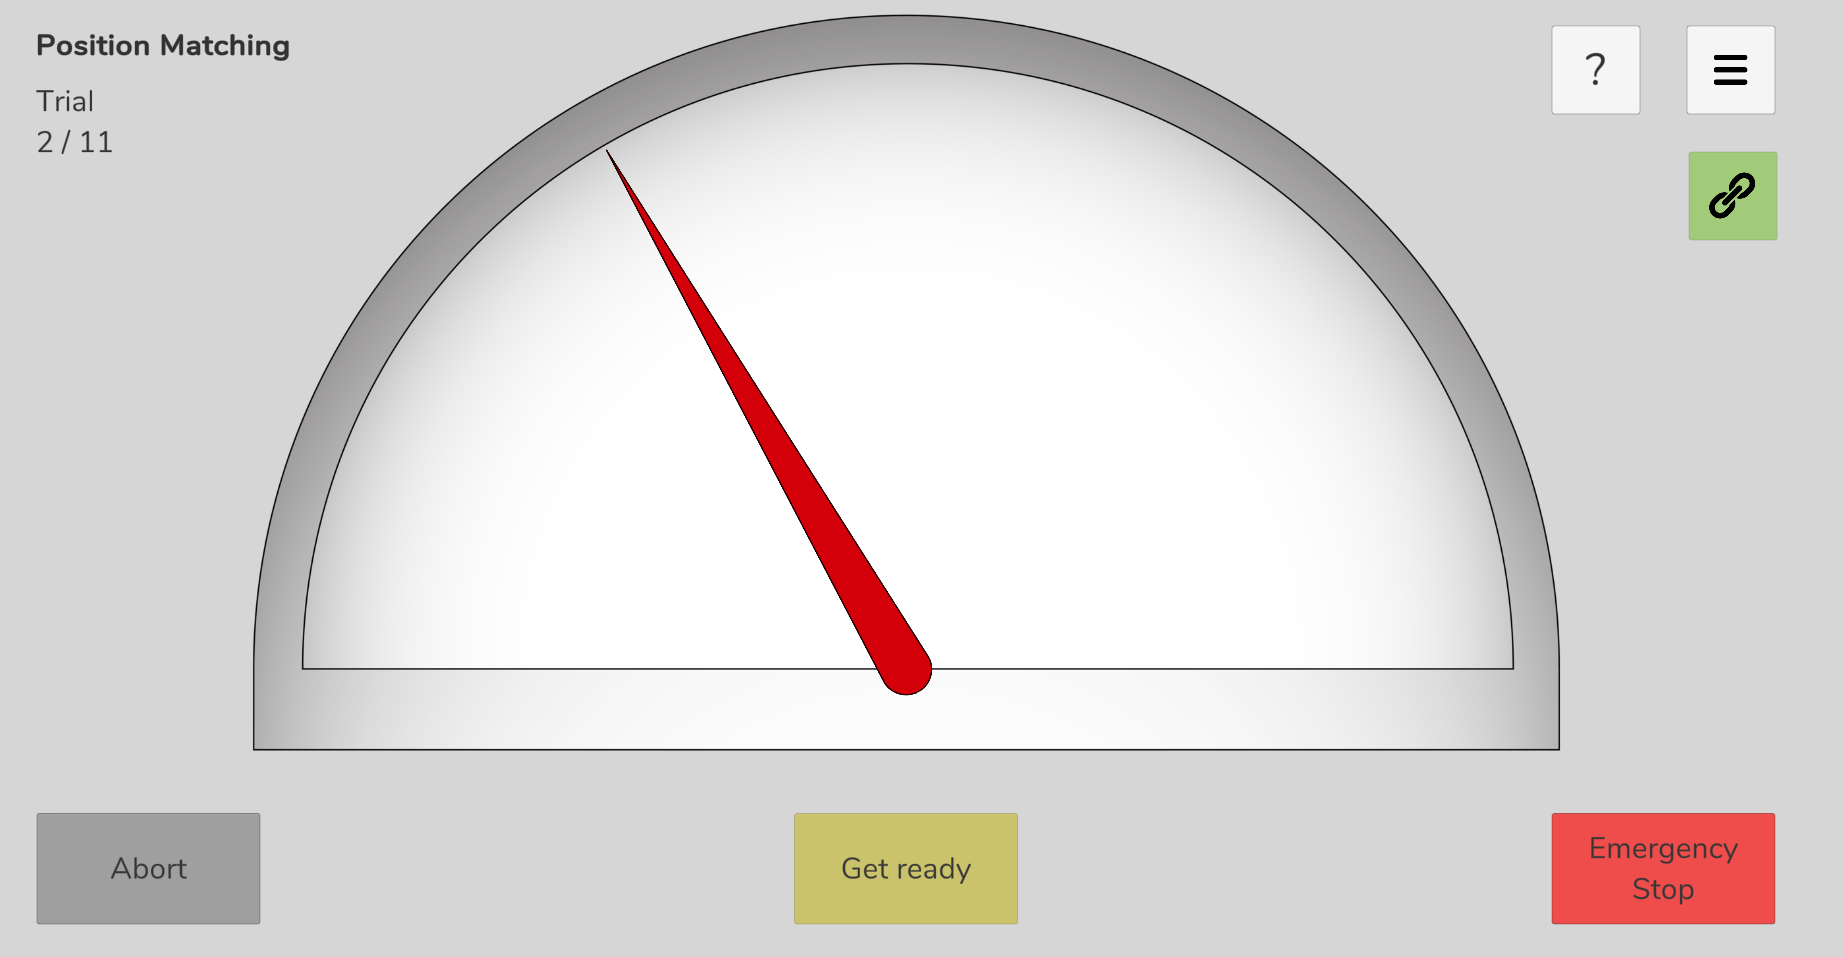
\includegraphics[width=\textwidth]{images/Assessments/PositionMatching1.png}
\end{subfigure}
\hfill
\begin{subfigure}[b]{0.48\textwidth}
	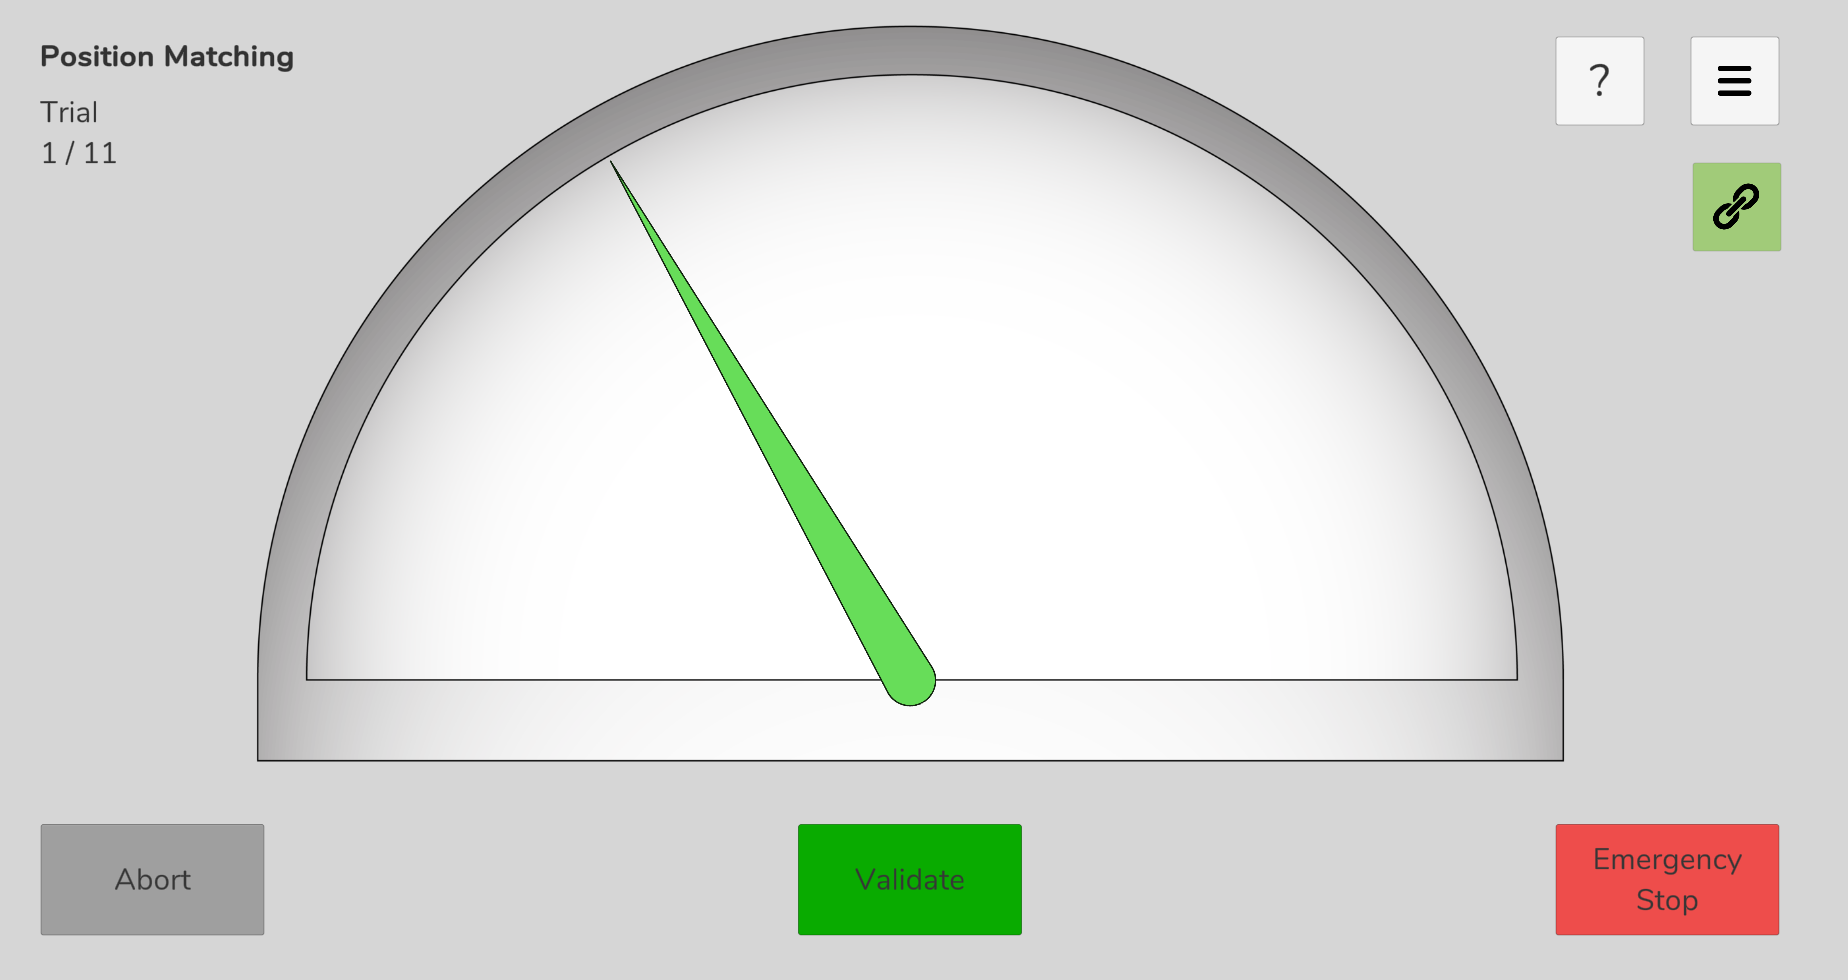
\includegraphics[width=\textwidth]{images/Assessments/PositionMatching2.png}
\end{subfigure}
\caption{Position matching task – the finger is automatically moved to the starting position by the robot (red gauge needle). Then, the finger is moved to another position and the subject needs to indicate, by dragging the green needle, the perceived finger position.}
\label{fig:PositionMatching}
\end{figure}

\subsection{Fast Reaching (motor impairments)}
The objective of this task is to move the finger as fast as possible from a starting position (red gauge needle) to the target (green gauge needle), as show in Figure \ref{fig:FastReaching}. The finger is first automatically moved to the starting position. As soon as the green needle appears, move towards it as fast as possible and keep your finger at it until the needle disappears again. Each trial lasts 4 seconds. The target will appear either in flexion or in extension direction. There are 10 repetitions. 

\begin{figure}[h!]
\begin{center}
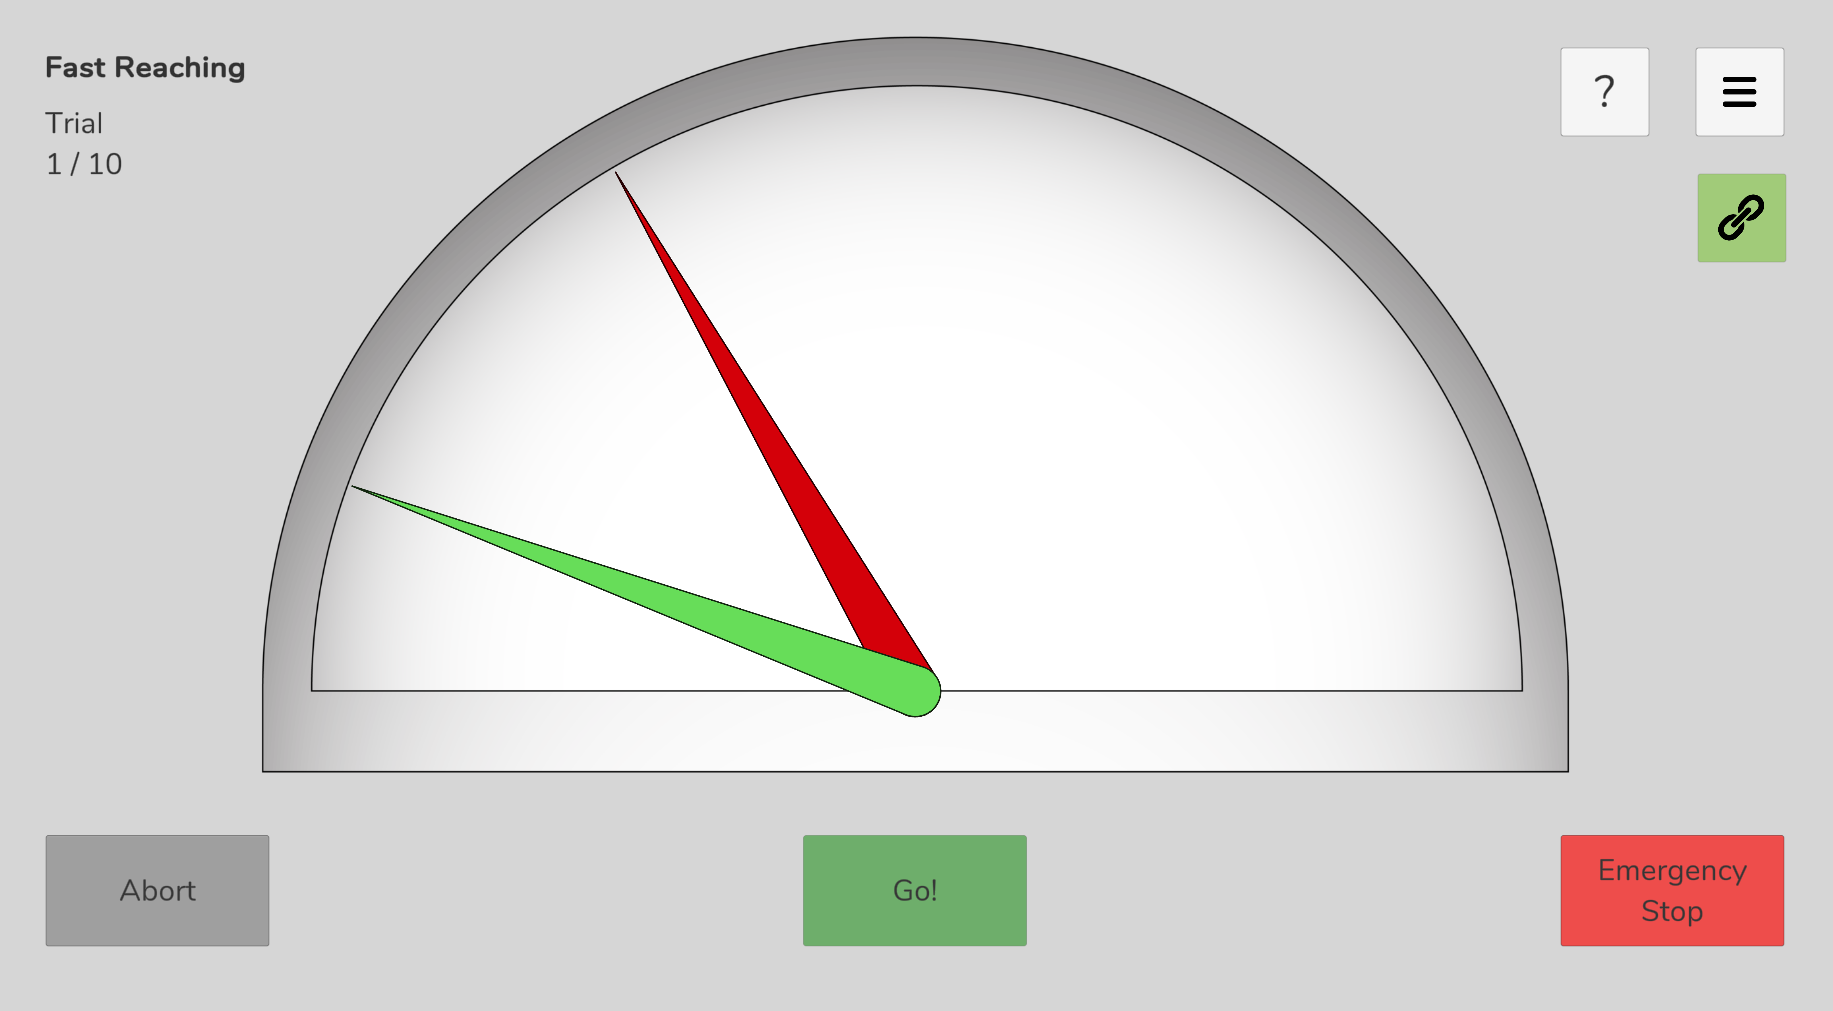
\includegraphics[width=0.7\columnwidth]{images/Assessments/FastReaching.png}
\caption{In the fast target reaching task, move your finger as fast as possible from the starting position (red needle) to the target (green needle).}
\label{fig:FastReaching}
\end{center}
\end{figure}

\subsection{Target Following (sensorimotor impairments)}
The objective of the task is to follow the target displayed on the screen as accurately as possible with your finger. The finger is first automatically moved to the starting position (red needle). Then, the red needle will disappear, and a green needle will appear, which will move slowly (see Figure \ref{fig:TargetFollowing}). Follow this trajectory as accurately as possible. Each trial lasts 30 seconds. There are 3 slow movement trials and 3 fast movement trials. 

\begin{figure}[h!]
\begin{center}
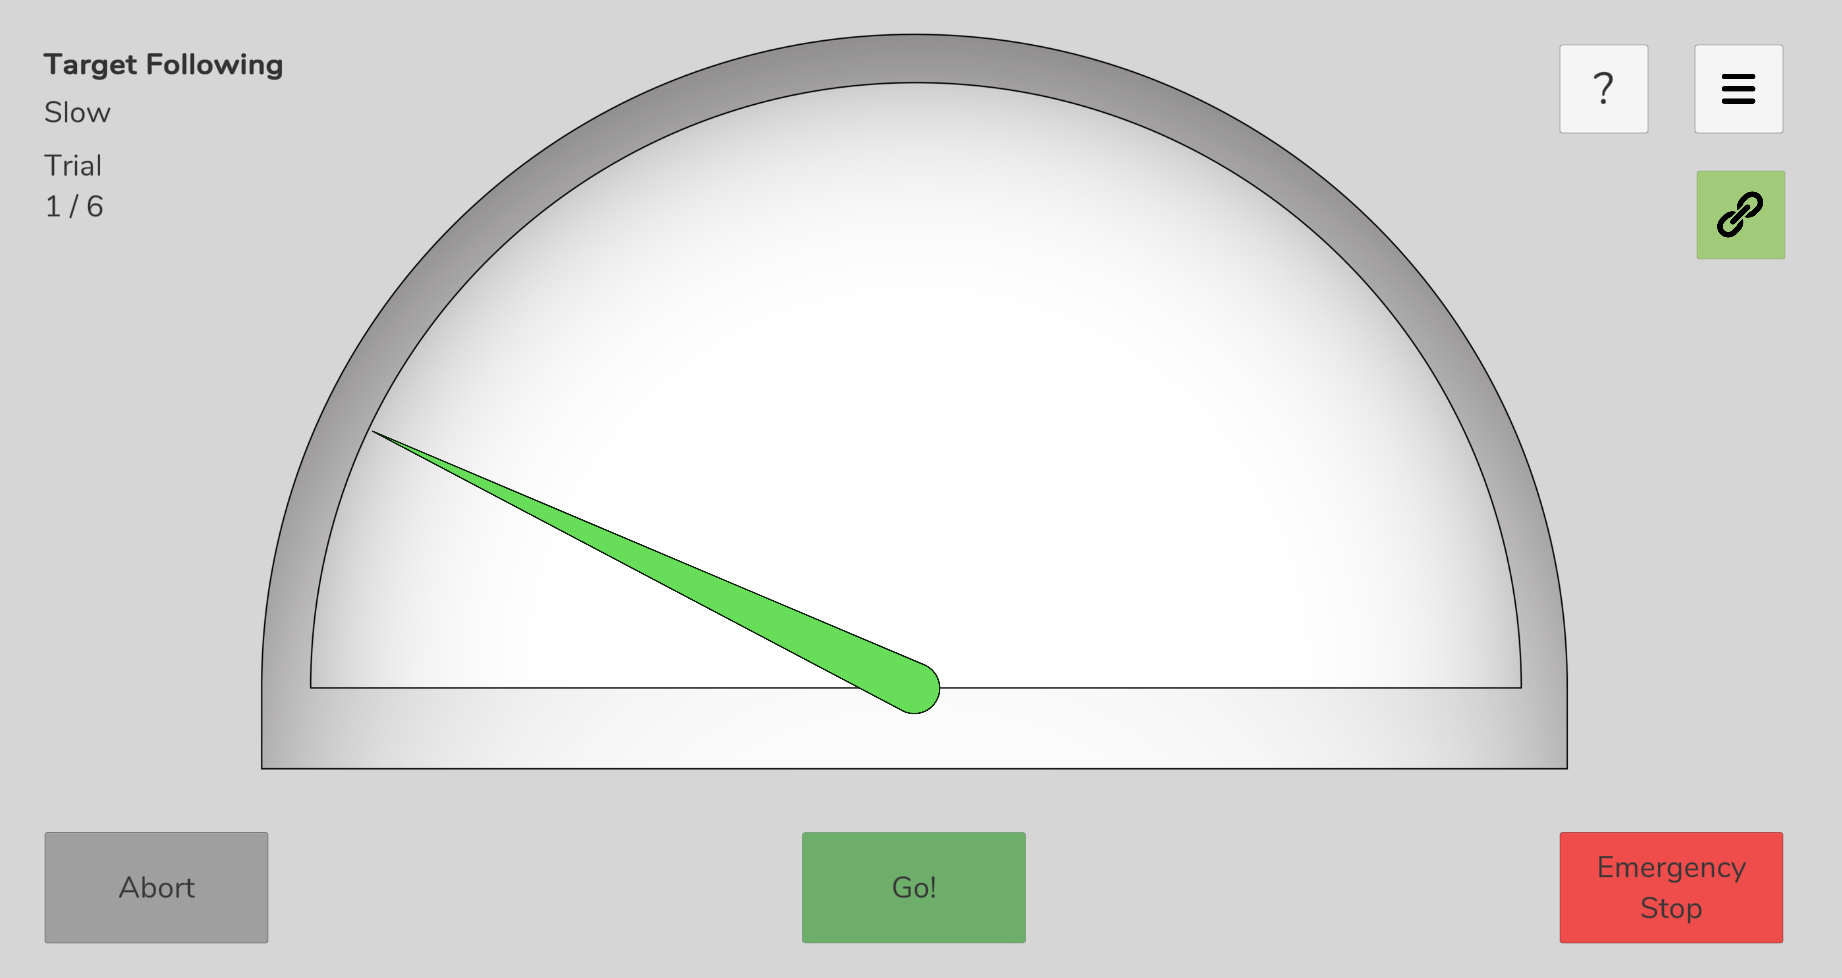
\includegraphics[width=0.7\columnwidth]{images/Assessments/TargetFollowing.png}
\caption{Target following task – follow the green gauge needle as accurately as possible.}
\label{fig:TargetFollowing}
\end{center}
\end{figure}

\subsection{Result Display}
\subsubsection{Results Summary per Hand}
In the task selection menu, in the bottom you can click \emph{Results Summary}, where all results are displayed (as in Figure \ref{fig:ResultSummaryHand}). These individual results can also be displayed directly after a task is performed (depending on the settings). In the Results Summary view, when you click on an individual window, the task display is enlarged and there you can see more details (e.g. Force Flexion or Force Extension). When you click on the small hand on the bottom of the display, you can switch between the display of the results for the left and the right hand. 

\begin{figure}[h!]
\begin{center}
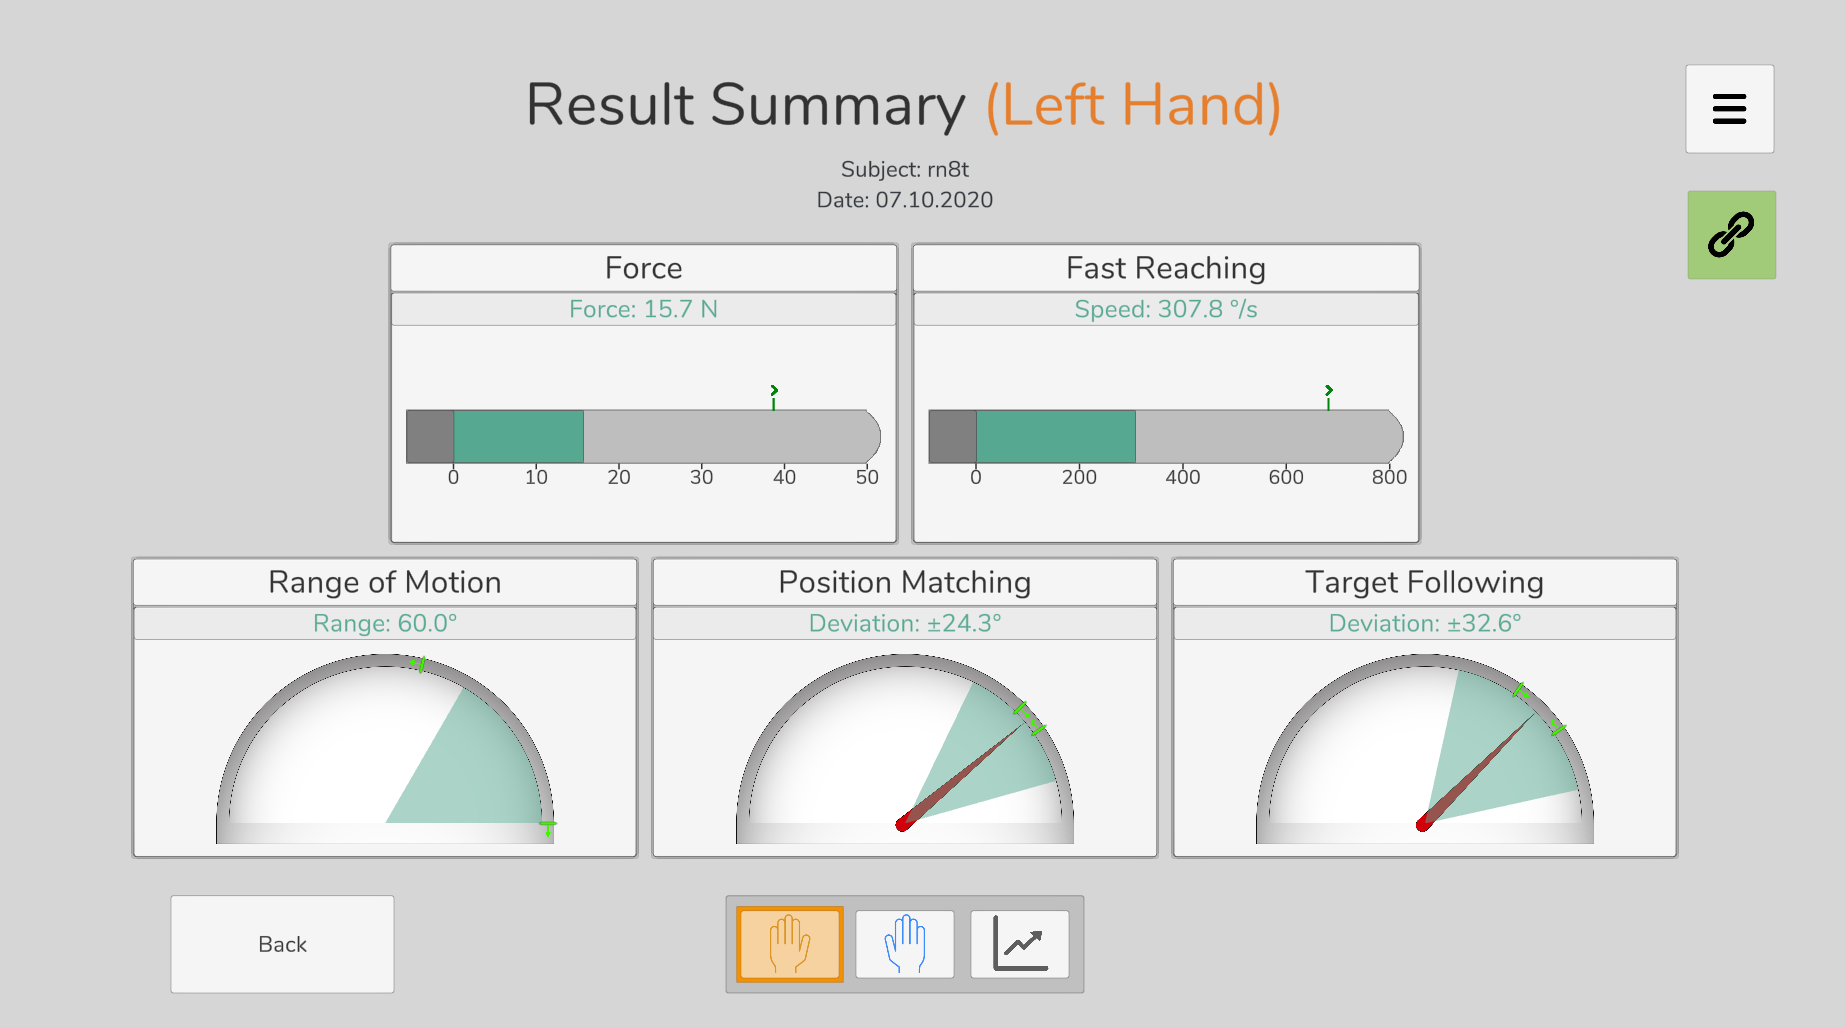
\includegraphics[width=\columnwidth]{images/Assessments/ResultsSummary.png}
\caption{Results summery per hand – click on an individual window to enlarge and see details.}
\label{fig:ResultSummaryHand}
\end{center}
\end{figure}

\subsubsection{Longitudinal Results Display} \label{sec:longResults}
With this view, you can see progress over time, in case you are performing the measurements in a longitudinal study (Figure \ref{fig:LongitudinalResults}). The x-axis displays assessment session number and y-axis the assessment task metric. Click on an individual window to enlarge and see details. The higher the values on the y-axis, the better the task performance (i.e. direction of improvement is pointing upwards).  

\begin{figure}[h!]
\begin{center}
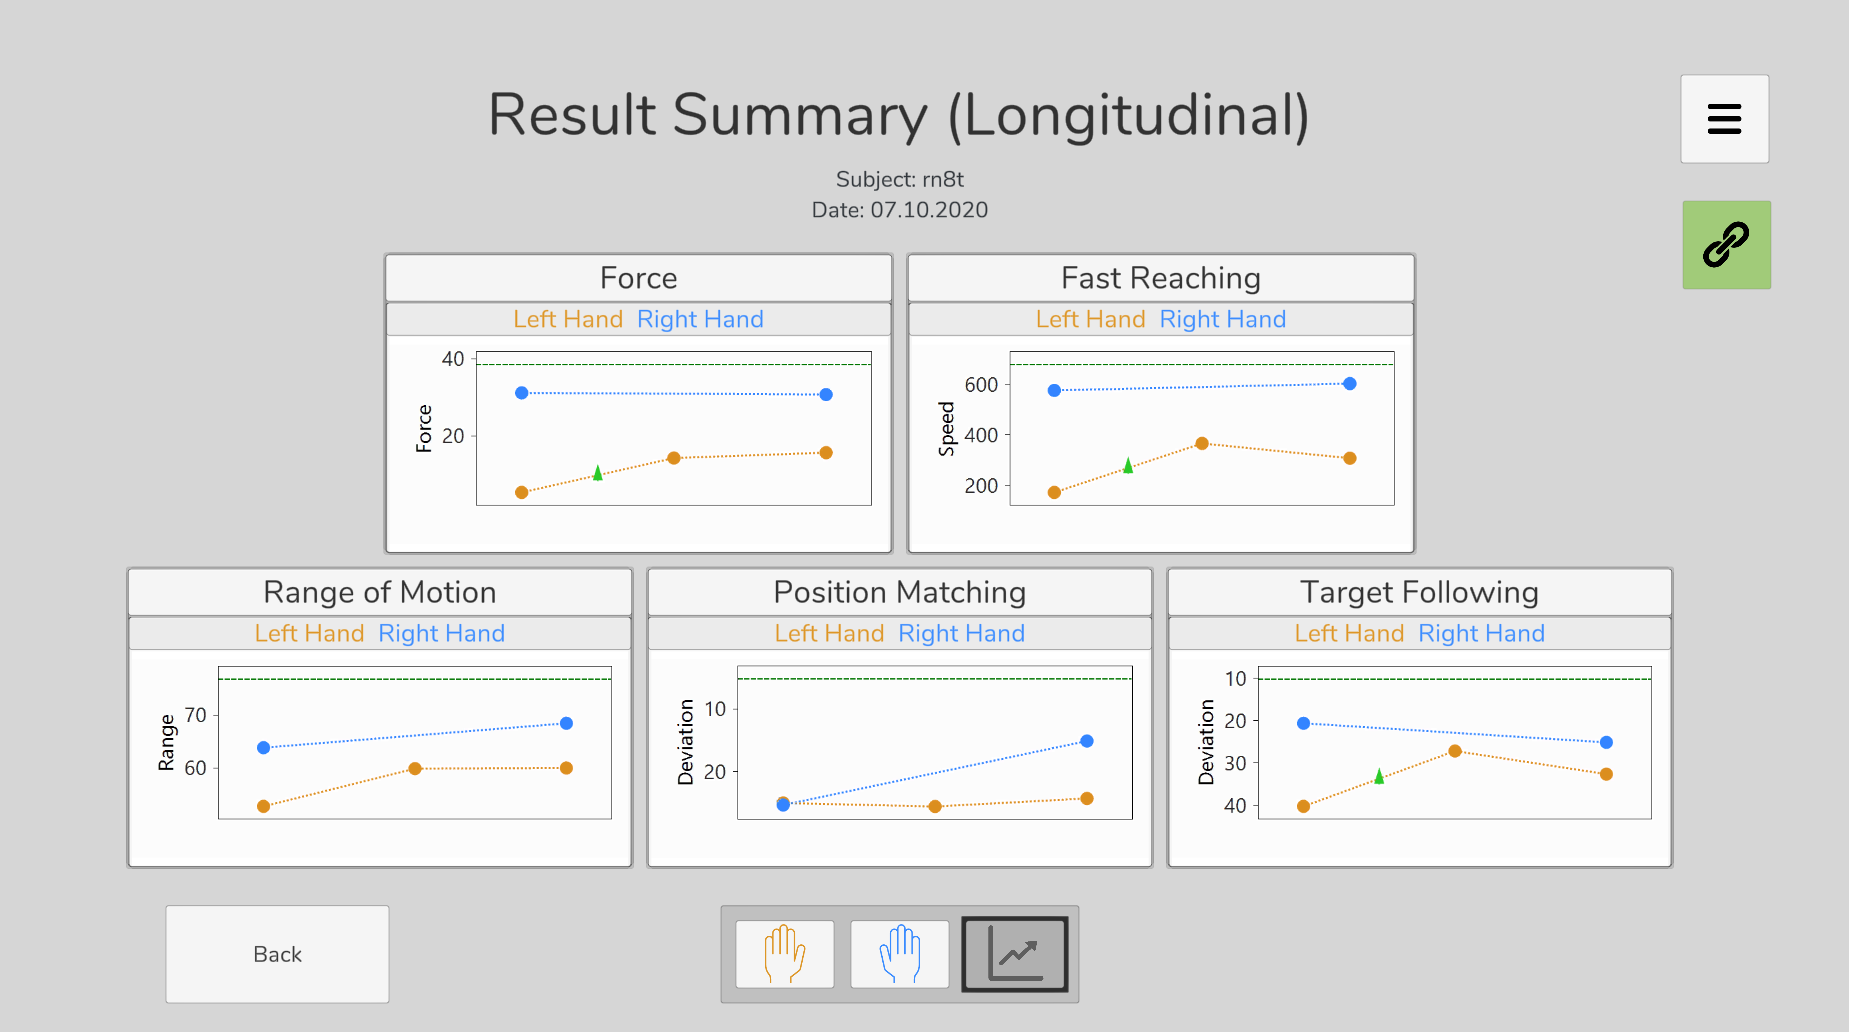
\includegraphics[width=\columnwidth]{images/Assessments/LongitudinalResults.png}
\caption{Longitudinal results summary. Click on an individual window to enlarge.}
\label{fig:LongitudinalResults}
\end{center}
\end{figure}

\newpage
\section{Data Storage}
\subsection{Raw Data}
The data is always stored under the subject ID that was automatically assigned to a new used that you created.
The data storage follows the structure indicated in Figure \ref{fig:RawData}, that is:
ETH MIKE xxx folder $\rightarrow$ Subject ID $\rightarrow$ Task Name (note: Motor Task $=$ Fast Reaching, Sensorimotor Task $=$ Target Following Task) $\rightarrow$ Hand $\rightarrow$ raw data (time stamp of when the measurement was started, practice rounds are market with practice).
TDMS file is preferred for data analysis, as this is coming directly from the sensors. The CSV files is what has been sent to the front-end over UDP, therefore there is a risk of small data package loss.
Additionally, Position Matching task contain \emph{.txt} file with target positions and indicated positions (this should be used for this task’s post-processing, as TDMS file doesn’t contain information on position indicated on the tablet).

\begin{figure}[h!]
\begin{center}
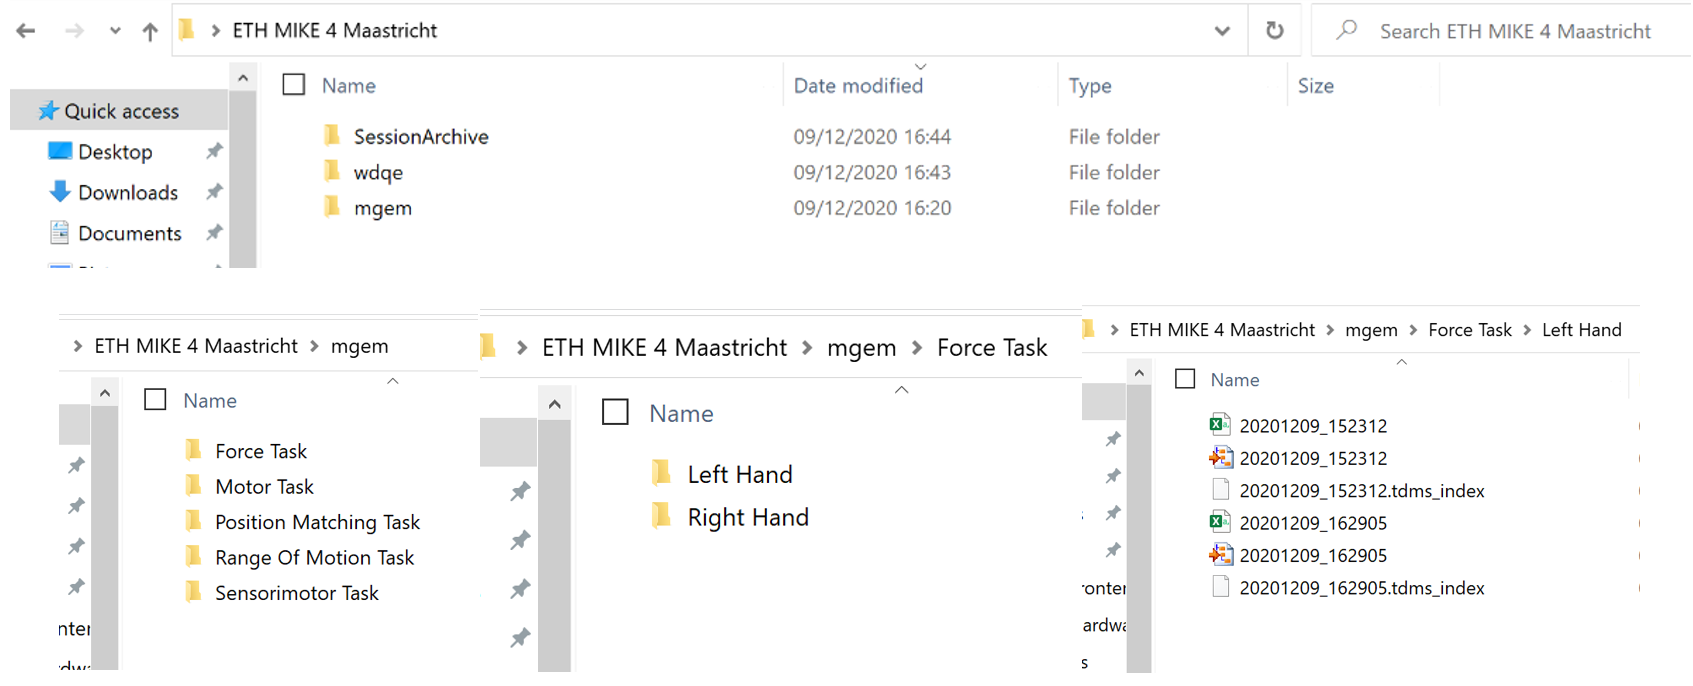
\includegraphics[width=\columnwidth]{images/TabletScreenshots/DataSaving.png}
\caption{Raw data saving – structure of the raw data storage folder.}
\label{fig:RawData}
\end{center}
\end{figure}

\subsection{Database}
Alternative way to access already processed data will be to open the SQL database, which is created as a basis for the longitudinal results display you saw in section \ref{sec:longResults}. The SQL database will allow you to easily access already processed data without the need to run post-processing on the raw data. However, the SQL database only contains the outcome measures that are displayed in the front end (one metric per task). If you would like to explore alternative metrics, you would need to work with the raw data. \\

To extract metrics from the database, first locate the file \emph{db.db} as indicated in Figure \ref{fig:DatabaseLocation}. You can then open it with \emph{DB Browser for SQLite}. This Software is already downloaded on the tablet, so it will automatically open when you double click on the \emph{db.db} file. To export results of task of interest (e.g. Force Task), follow the steps indicated in Figure \ref{fig:SQLDatabase}. 

\begin{figure}[h!]
\begin{center}
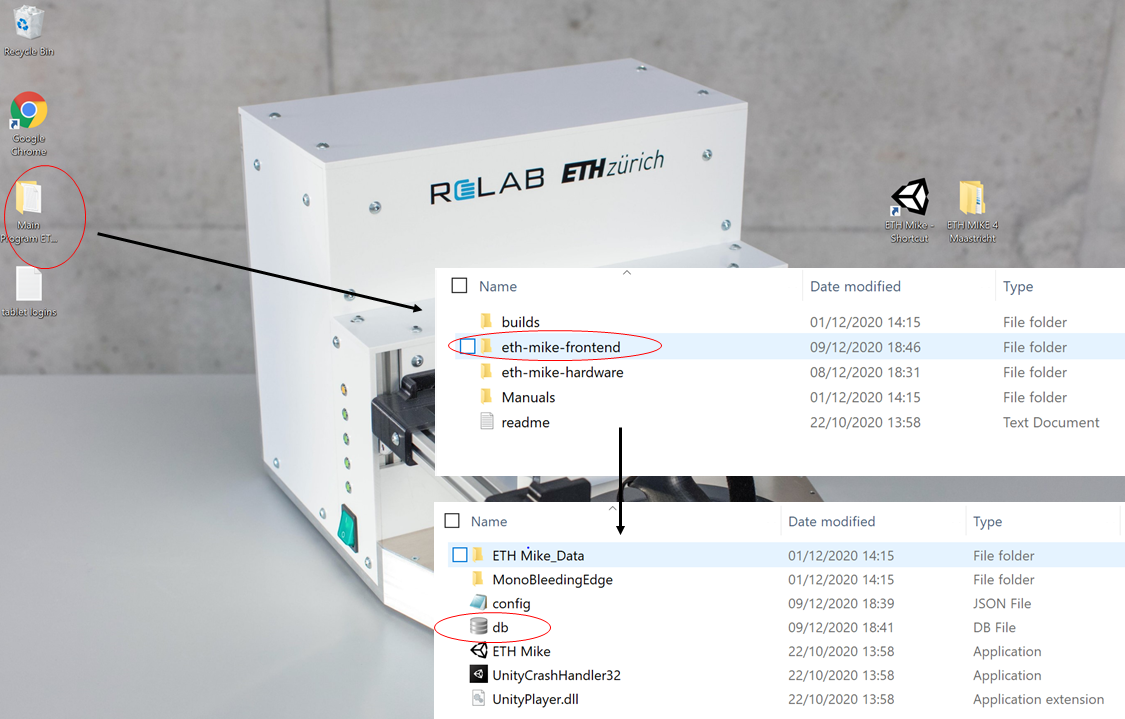
\includegraphics[width=\columnwidth]{images/TabletScreenshots/Database.png}
\caption{Location of the database with calculated metrics for each task.}
\label{fig:DatabaseLocation}
\end{center}
\end{figure}

\begin{figure}[h!]
\begin{center}
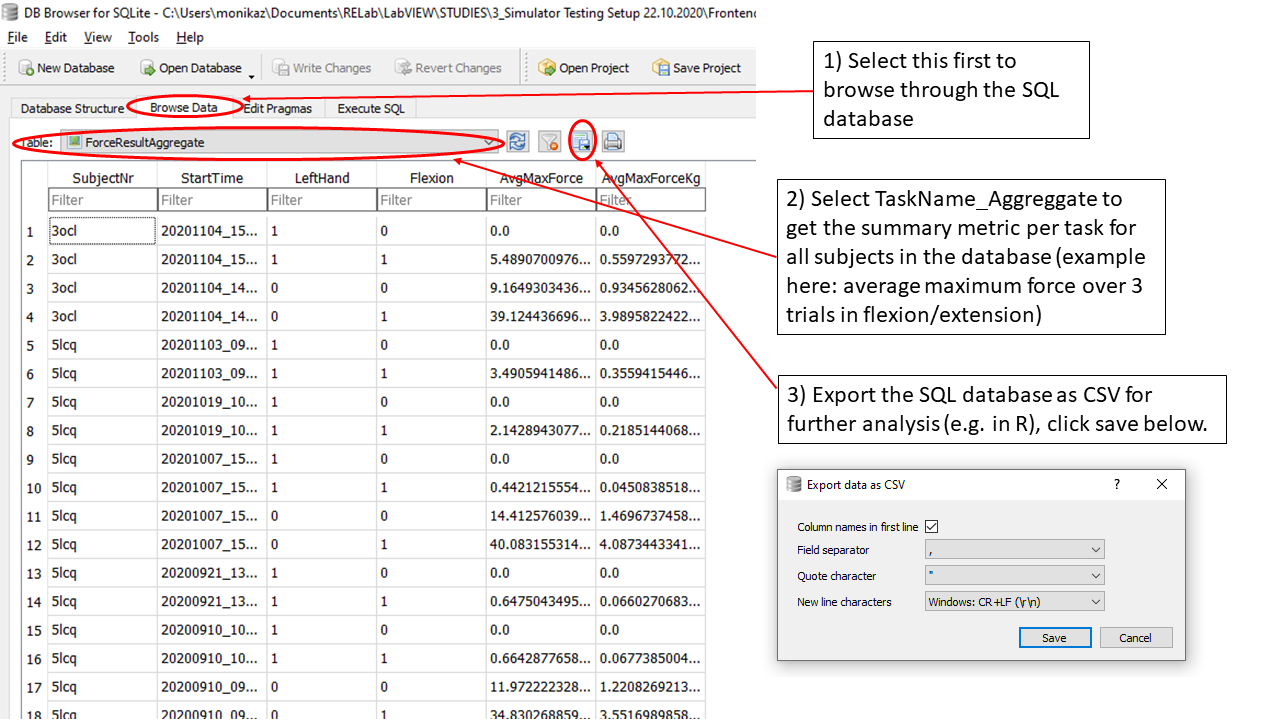
\includegraphics[width=\columnwidth]{images/TabletScreenshots/ExportDatabase.png}
\caption{How to browse a SQL database and export results of a task in CSV.}
\label{fig:SQLDatabase}
\end{center}
\end{figure}

\newpage
\phantom{blabla}
\newpage
\section{Packing for Transportation}
Follow the steps indicated in Figure \ref{fig:Packaging} to pack or unpack the robot safely. The white foam is durable and can be reused for packaging and transporting the robot multiple times.\\

The robot needs to be placed in a box of \SI{50x50x70}{\cm}. First, place the robot, with its end-effector fixated with the end-effector lock (the screw can be slightly tightened for transportation using an Allen key), inside the box (\#1 and \#2). Then, cover the end-effector with the bubble wrap. Cover larger components (handles and safety stop) in bubble wrap and place it under the tablet rails (\#3). Tablet and its keyboard, placed inside a box, should be covered in the bubble wrap and placed at the back of the robot (\#3). Then, place a foam protection above the tablet rails (\#4). Next, place all cables and small components into their designated box and cover it with bubble wrap. Also cover the incline place in bubble wrap. Place the box with cables and the incline plane on top of the foam (\#5). Place two protective pieces of foam (\#6). Close the box, then wrap it in bubble wrap and place inside a bigger box for transportation (\SI{57x57x77}{\cm}). This step is only necessary for shipment. The total weight of the system is around \SI{20}{\kg}. 

\begin{figure}[h!]
\begin{center}
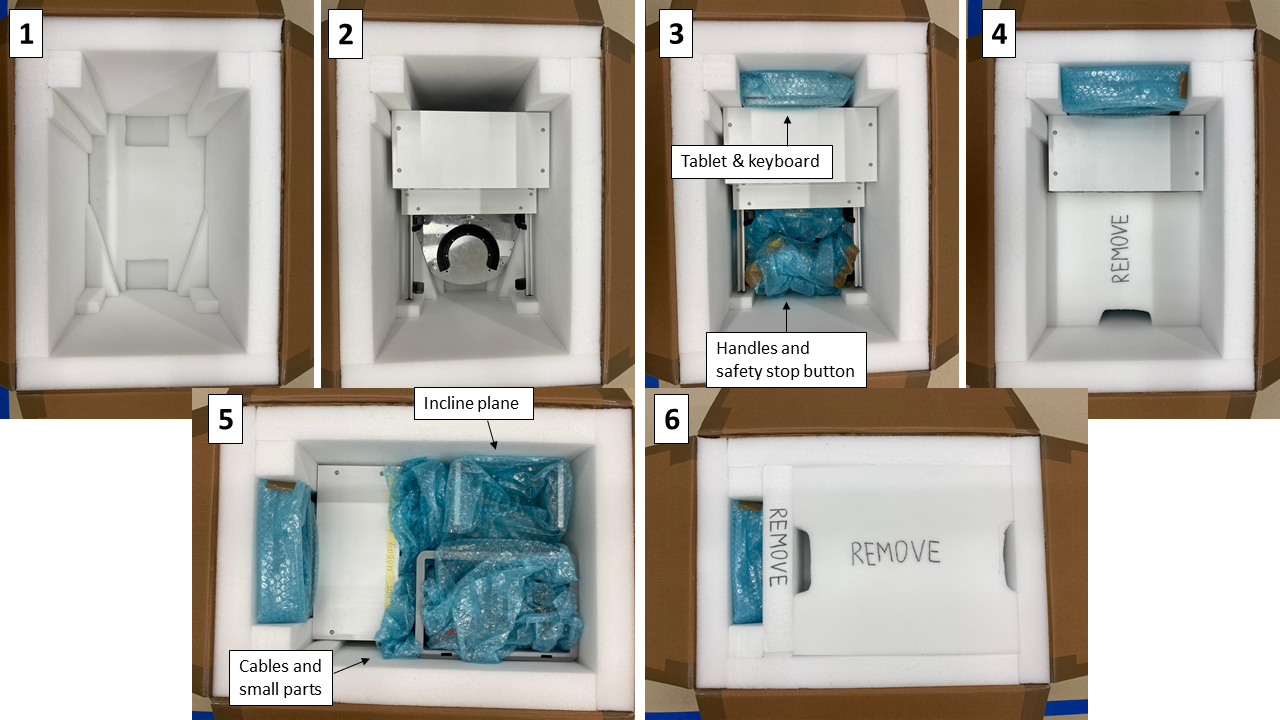
\includegraphics[width=\columnwidth]{images/Box/Packaging.png}
\caption{How to pack the robot safely.}
\label{fig:Packaging}
\end{center}
\end{figure}
\newpage
\section{Troubleshooting}
Below you will find a description of possible issues and how to solve them. 

\subsection{Software Disconnects from Hardware}
Follow the steps below to address the issue: 

\begin{enumerate}
\item Make sure that the USB cable is connected (connecting the robot with the tablet). 
\item Restart the robot hardware (turn the switch located on the side of the robot off and on again). Don’t forget to place the end-effector in the middle when turning the robot on. 
\item Software: If you are in \emph{Task Selection}, click on the \emph{Main Menu} button and there select \emph{Logout}. Wait for the connection icon to turn green. Once it runs green and if you were not finished with last session, click \emph{Resume last session} instead of starting a new session (\emph{New Session}). Use the same subject code you were using when the robot disconnected.  
\item If the robot disconnects during an assessment, go back to Task Selection (click \emph{Abort}) and wait until the icon turns green. Then repeat the assessment that was interrupted. 
\item If the icon doesn’t turn green after you have tried steps 1-4, close the application (click \emph{Quit} in \emph{Main Menu}). 
\item Restart the robot again. 
\item Open the application.  Insert subject code and click \emph{Resume last session}.
\end{enumerate}

\begin{figure}[h!]
\begin{center}
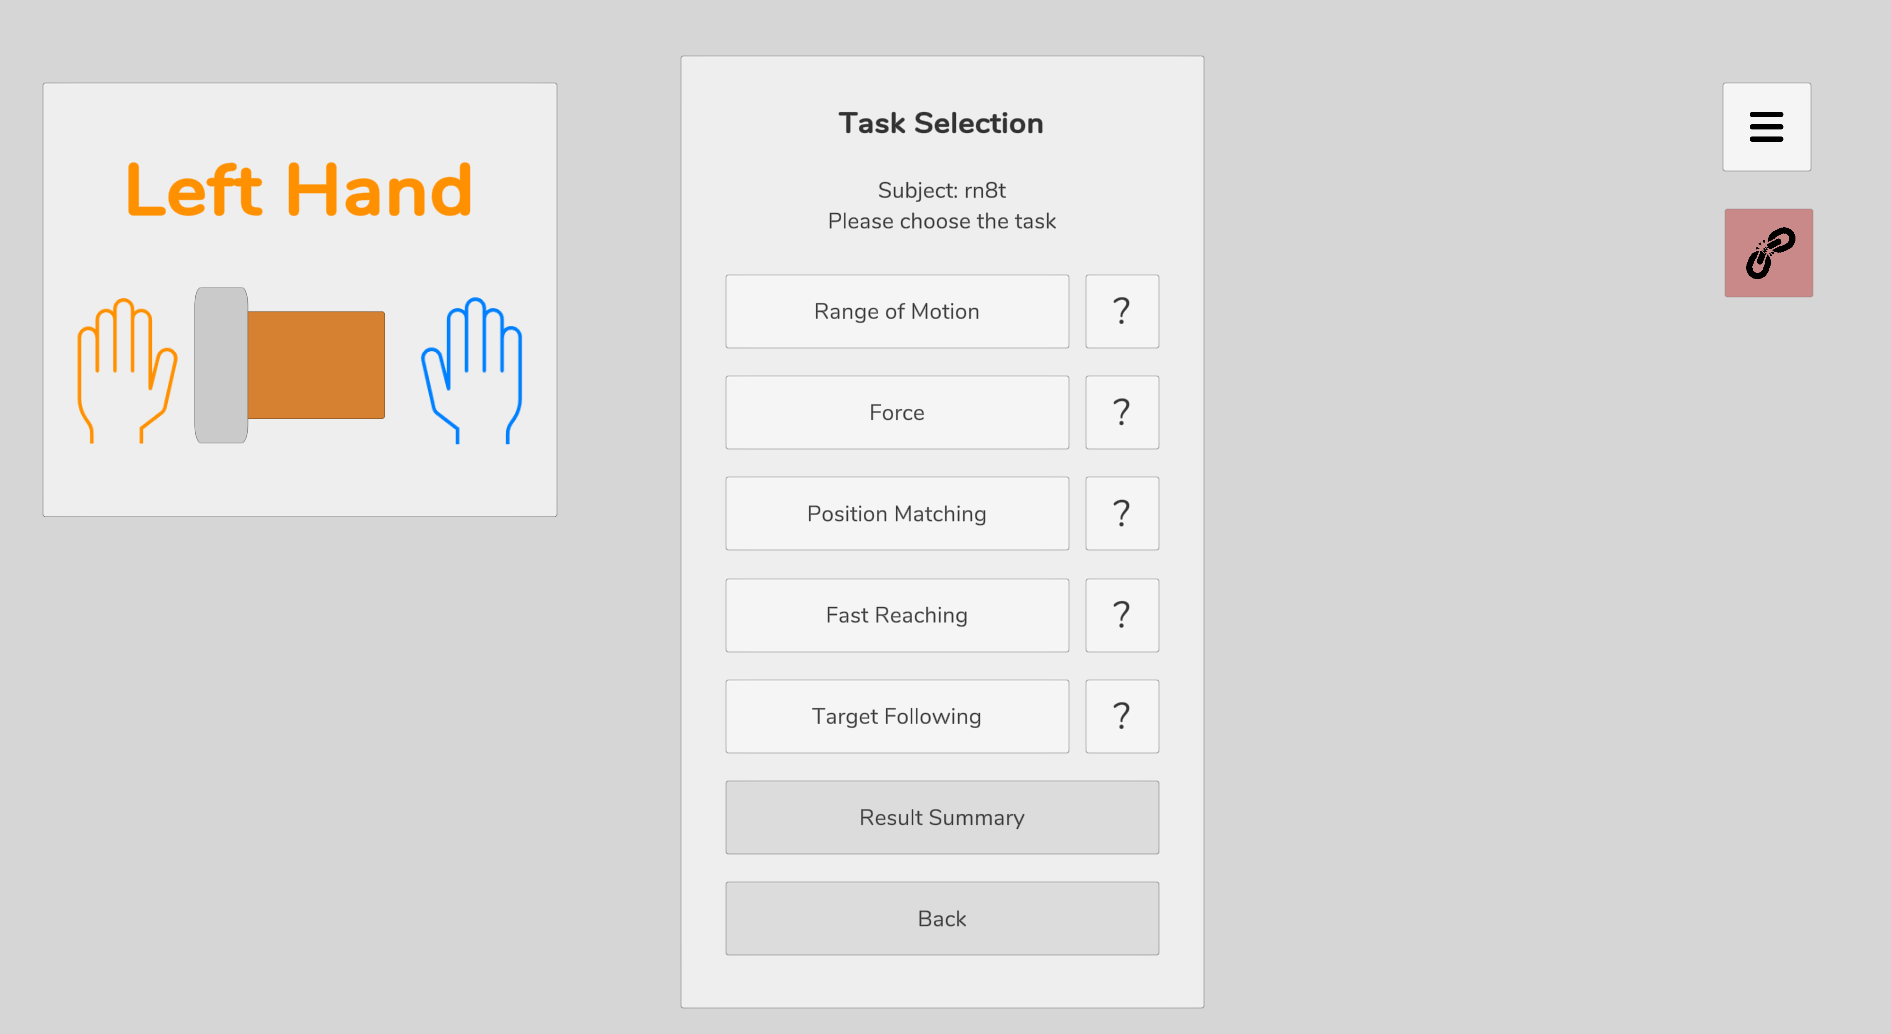
\includegraphics[width=\columnwidth]{images/Troubleshooting/SoftwareDisconnects.png}
\caption{In case connection between software (tablet) and hardware (robot) gets lost/disturbed, you will see the icon on the right appearing “broken” and in red colour.}
\label{fig:Disconnection}
\end{center}
\end{figure}

\subsection{Software crashes}
In case the software application suddenly closes, open it again and you will see the pop-up as in Figure \ref{fig:Crash}. Confirm with \emph{Yes} that you would like to continue, and you will get back to where you were before the shutdown.

\begin{figure}[h!]
\begin{center}
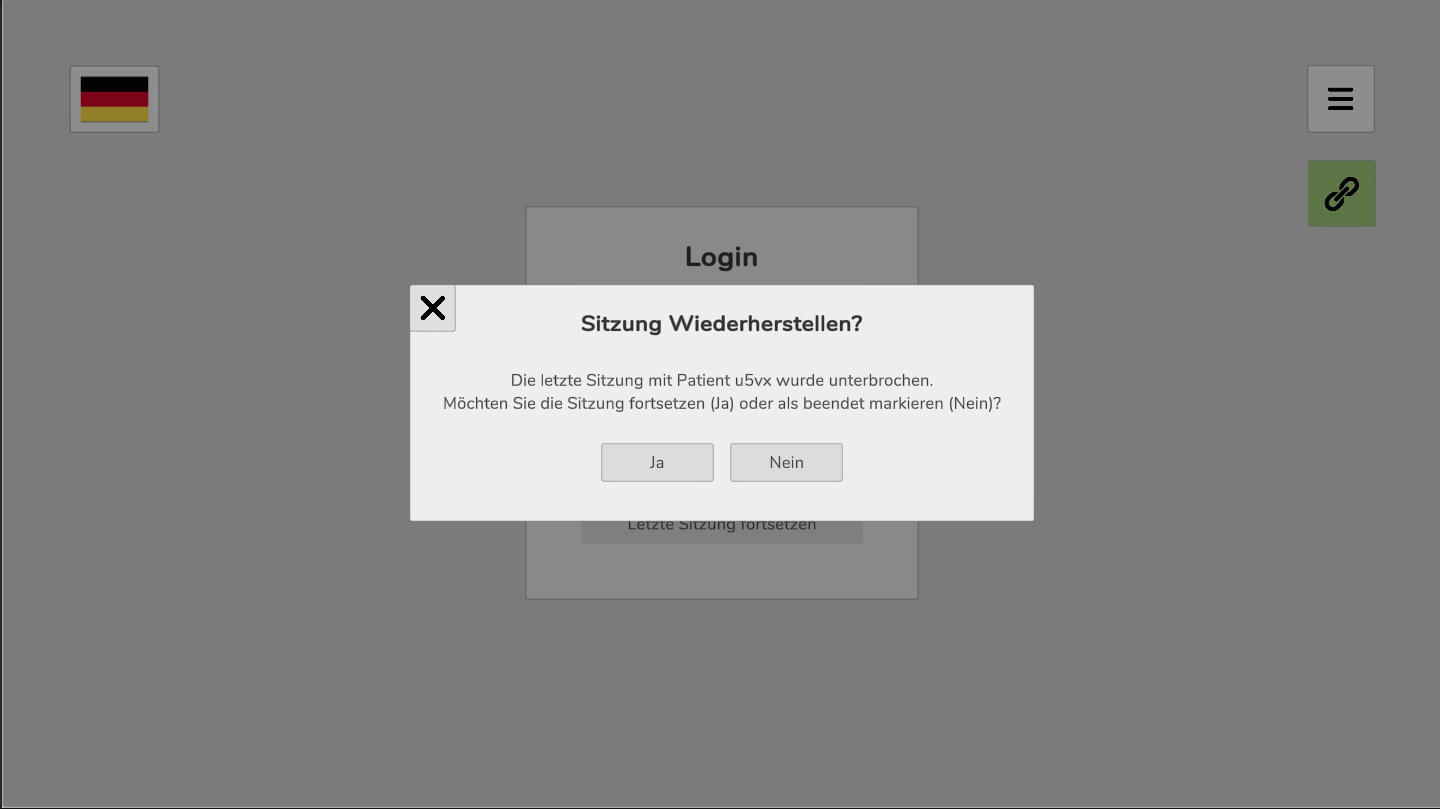
\includegraphics[width=\columnwidth]{images/Troubleshooting/SoftwareCrash.png}
\caption{Pop-up that appears when reopening the application after a software crash.}
\label{fig:Crash}
\end{center}
\end{figure}

\newpage
\section{Contact Information}
Monika Zbytniewska\\
Rehabilitation Engineering Laboratory\\
ETH Zurich\\
BAA, Lengghalde 5\\
8008 Zurich\\
+41 779 615 277\\
monika.zbytniewska@hest.ethz.ch\\
\href{http://www.relab.ethz.ch}{http://www.relab.ethz.ch}\\

Olivier Lambercy\\
Rehabilitation Engineering Laboratory\\
ETH Zurich\\
BAA, Lengghalde 5\\
8008 Zurich\\
+41 44 510 7246\\
olivier.lambercy@hest.ethz.ch\\
\href{http://www.relab.ethz.ch}{http://www.relab.ethz.ch}\\





\end{document}